% chapter3 模型

\chapter{基于脑电图信号的运动想象脑电图分类网络构建}

论文前两个章节主要对运动想象脑电图(Motor Imagery Electroencephalography,MI-EEG)分类领域的基础知识以及相关研究做了一定的介绍,并且对该领域仍然存在的问题进行了分析。本章对这些问题进行进一步的探讨,针对这些问题进行了以下研究:

(1) 针对运动想象脑电图分类任务精度有待提升的问题,构建了一种端到端的新模型HIT-Net:首先,以ShallowConvNet模型为基础,引入多尺度并行特征提取模块(Inception模块)\cite{szegedy2015going}、瓶颈层、深度可分离卷积和混合注意力机制,旨在并行提取多尺度时间特征,促进时空特征的深度融合,同时提高模型对重要特征的关注度;其次,在以上模型的基础上,将密集连接引入Inception模块的分支中,以更好地利用EEG信号的局部细节和浅层特征;最后,引入并行多分支的Transformer模块以更好地利用EEG信号的全局信息,并且针对EEG信号信噪比低的特点,引入软阈值模块对Transformer进行改进,从而减少噪声的干扰。

(2) 针对运动想象脑电图分类任务即时响应的需求,对HIT-Net进行了轻量化设计,构建了一种紧凑型端到端模型VSNet:首先,删去参数量较大的Inception模块和Transformer分支,保留网络的其他结构;其次,使用单层的深度可分离卷积替代Inception模块作为时间卷积层,并对瓶颈层进行调整。

(3) 针对运动想象脑电图缺乏标注数据的问题,设计了一种半监督的迁移学习算法:首先,通过ICA算法和Wasserstein距离\cite{rubner2000earth}选择与目标域分布相似的N个源域;其次,将源域与目标域的特征在黎曼流形上对齐并映射到切线空间,并通过源域与目标域特征的相似性计算特征的权重;最后,基于MEKT算法获取特征映射矩阵,并通过加权投票获取最终的结果。

本章分三个部分对这些研究进行介绍。

\section{基于Inception和混合注意力融合改进的端到端MI-EEG分类网络HIT-Net}

原始的EEG信号通常为二维数据,包括通道(电极)和时间两个维度,具体而言,在EEG信号矩阵中,行代表分布在头皮不同位置的采样通道,列为时间序列数据,每个采样点对应一个时间戳下的生物电信号(通常为电压值),因此,一列数据就是一个特定时间点下所有通道同步采集到的电压读数。原始的EEG信号经过预处理之后,可以转换为时频图、头皮点位拓扑图等输入模式,尽管经过转换的输入相较于原始输入能够更全面地体现EEG信号的时频空信息,但这一过程往往需要具有神经科学背景的人工参与,在增加了人工成本同时,限制了模型自适应学习EEG信号中蕴含的复杂时空特征的能力,此外,复杂的预处理环节也增加了计算开销和应用成本,难以满足BCI系统即时响应的需求。因此,端到端网络在MI-EEG分类领域受到越来越多的重视,这类网络不经过或者仅仅经过很少的预处理步骤,而由深度学习算法自适应地提取关键特征并作出预测。

为此,论文构建了基于Inception和混合注意力融合改进的端到端MI-EEG分类网络HIT-Net(HybridAttention-Inception-Transformer-MI-EEGNet),其结构如图~\ref{fig:HIT}~所示。HIT-Net有两条并行分支,分别是卷积神经网络分支与Transformer分支。卷积神经网络分支基于Inception结构搭建,通过在Inception分支引入密集连接结构,进行多尺度特征提取,同时利用高级语义信息与浅层特征;通过引入反转瓶颈层,在深度维度上促进时空特征的融合,同时通过深度可分离卷积等方法减小网络的参数规模;通过引入svSE混合注意力模块促进网络对重要特征的关注度,svSE模块采取时空特征分离的策略,同时利用了EEG信号的方差信息,以获得针对性的结果。Transformer分支用以获取全局上下文信息,同时采用了时空特征分离的策略,以并行分支方式进行通道上的时间长距依赖信息;通过引入软阈值函数以抑制噪声。卷积神经网络分支与Transformer分支通过CT-Block与TC-Block进行特征的融合,以同时利用Transformer提取的全局信息与卷积神经网络提取的局部细节,构建长短依赖的混合注意力机制。

通过HIT-Net,可以更完整地获取MI-EEG信号的有效特征,提升分类效果。在下文中,将依次阐述论文的改进思路与构建方法。

\begin{figure}
    \centering
    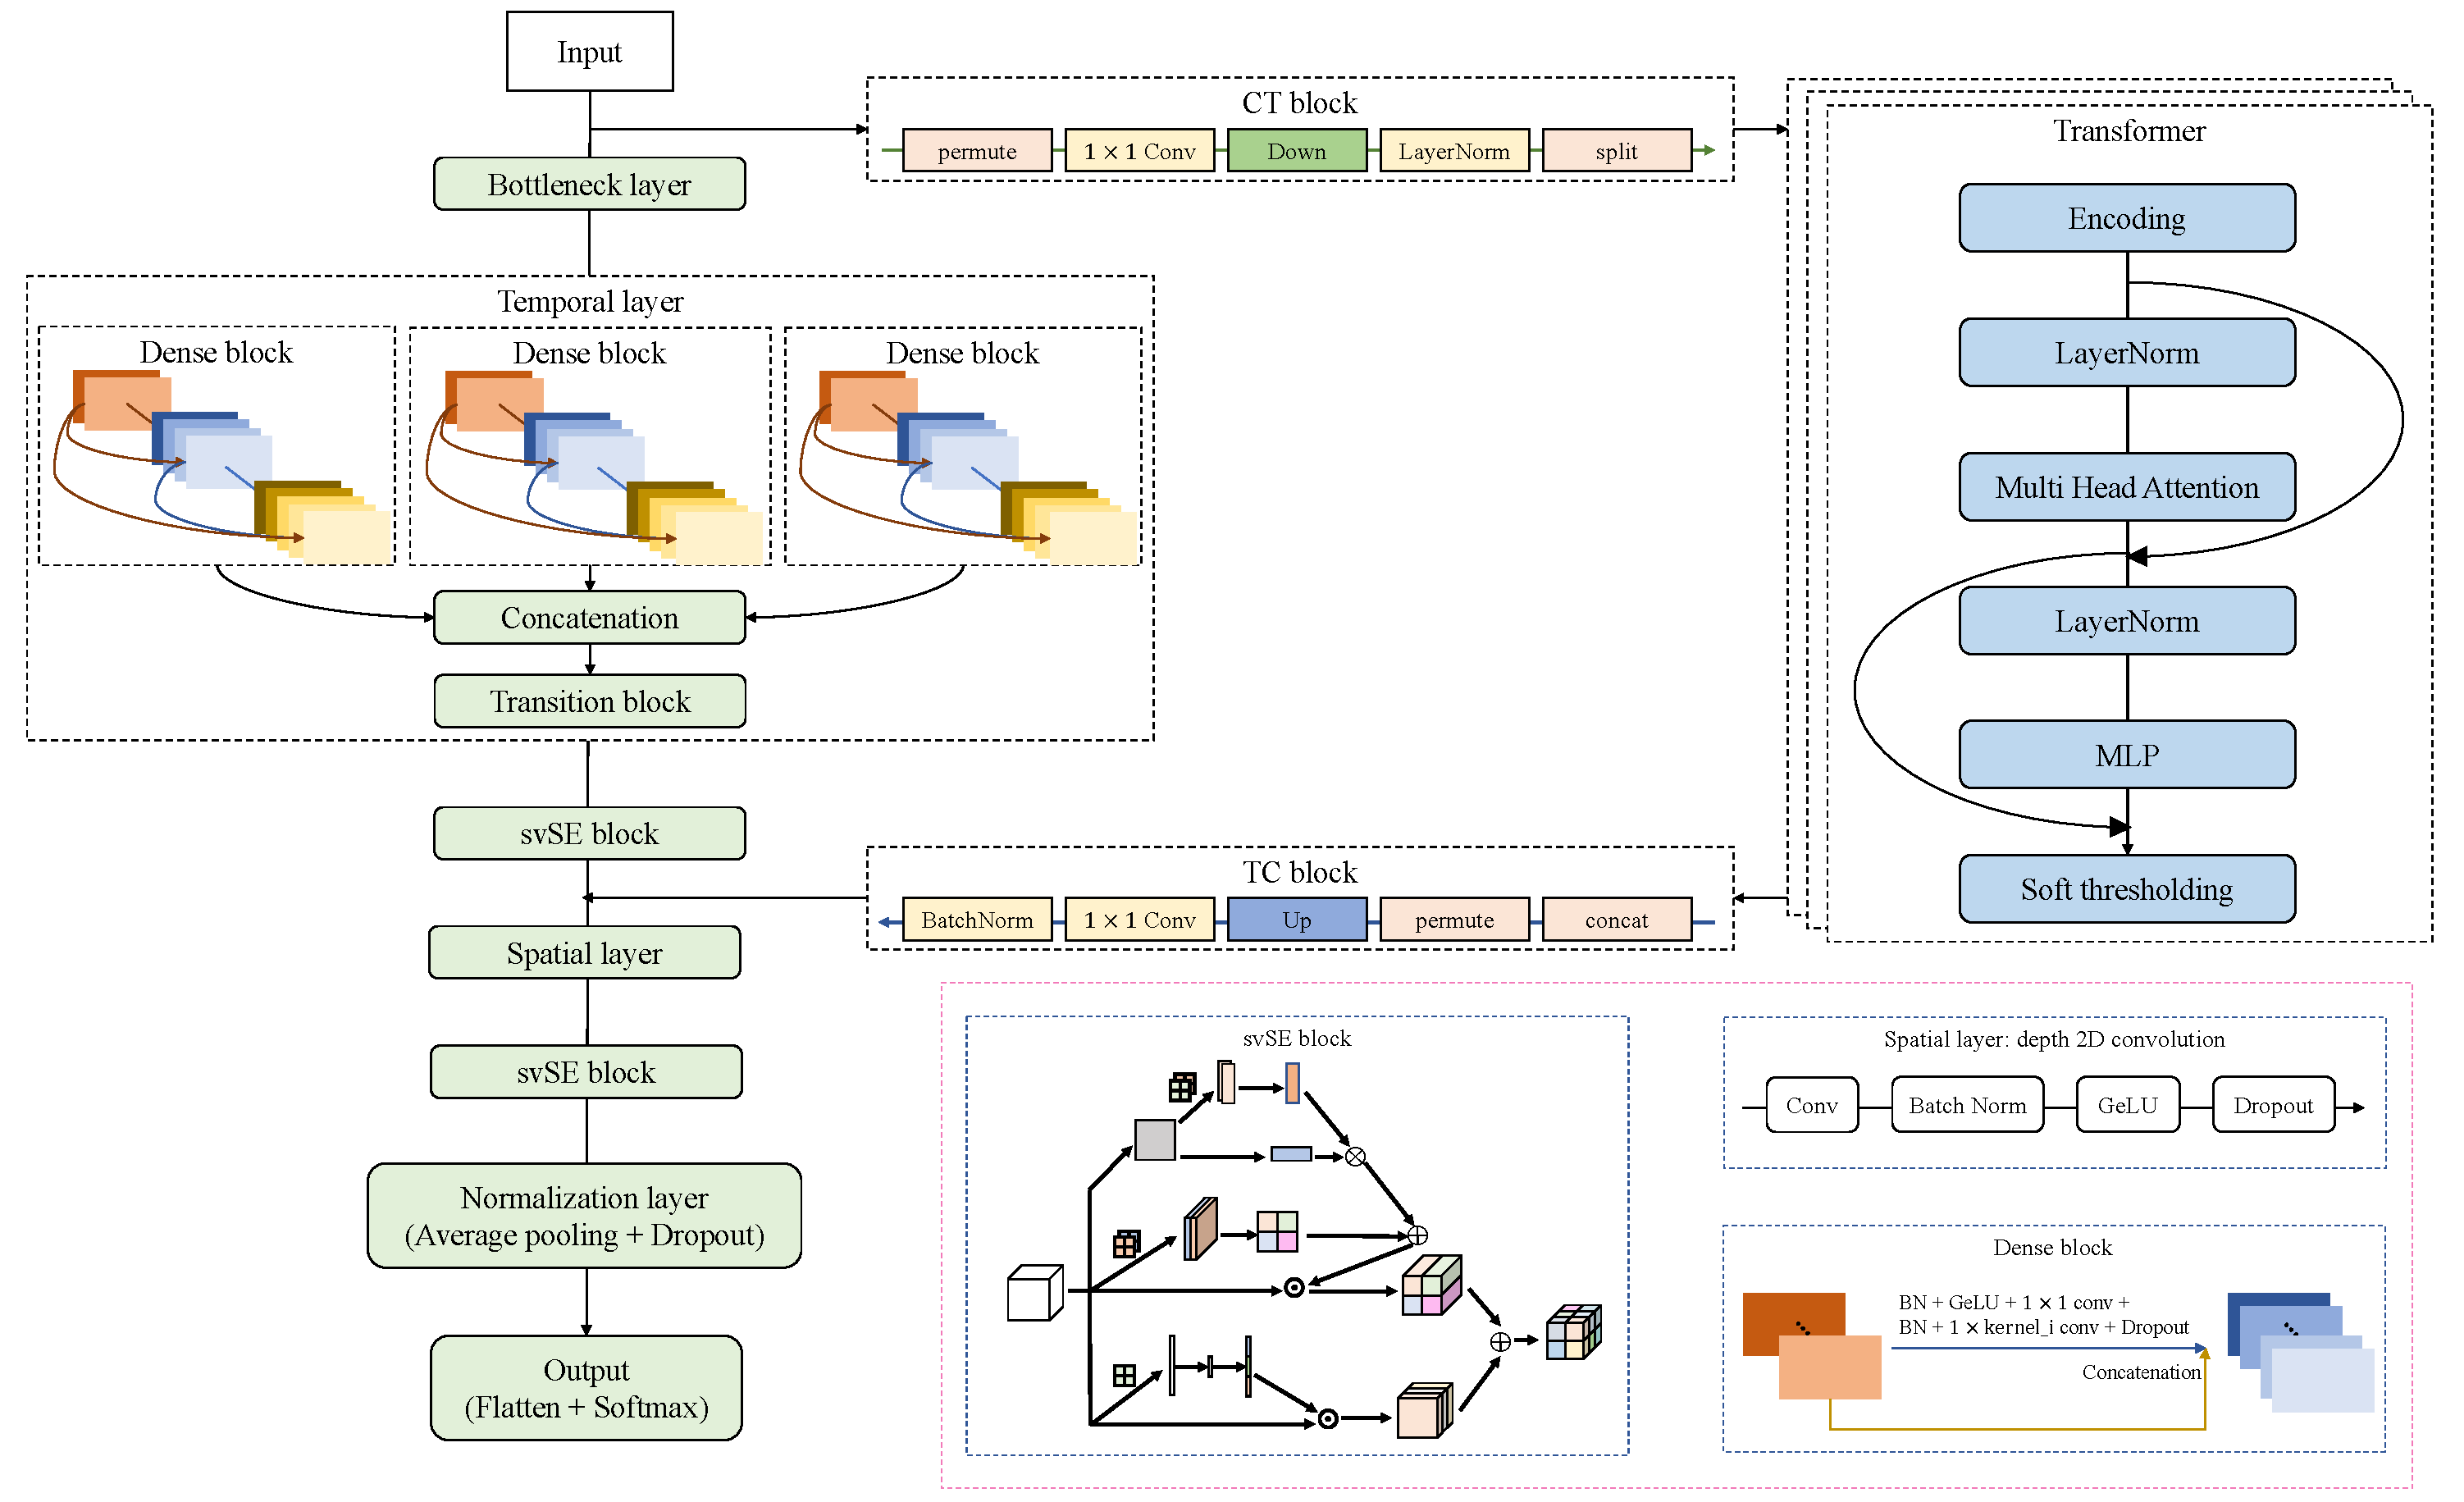
\includegraphics[width=\textwidth]{HIT-Net.pdf}
    \caption{HIT-Net结构}
    \label{fig:HIT}
\end{figure}

\subsection{基础网络BaseNet}

ShallowConvNet\cite{schirrmeister2017deep}是一个专为端到端解码脑电图(EEG)信号而设计的深度学习架构,其构思源自EEG信号解码研究领域中广泛使用的经典特征提取方法——滤波器组共空间模式(Filter Bank Common Spatial Pattern, FBCSP)\cite{ang2008filter}。ShallowConvNet具有FBCSP算法对频带功率特征高效提取的特性,在实验中证明了能够学习频带功率变化的时间结构特性\cite{schirrmeister2017deep},研究发现,该特性有助于提高分类性能\cite{sakhavi2015parallel}。实验证明,ShallowConvNet在MI-EEG分类领域具有优良的性能\cite{lawhern2018eegnet},同时具有较少的参数量,因此论文参考ShallowConvNet设计MI-EEG分类网络。

ShallowConvNet的结构如图~\ref{fig:ShallowConvNet}~所示。ShallowConvNet采用四步流程对原始二维输入数据进行处理。具体而言,ShallowConvNet首先通过时间卷积层捕获信号的时间域特征,再通过空间卷积层捕获这些时间特征在不同通道间的空间关联性,随后通过平均池化层进行下采样,最后通过全连接层将多维特征映射至分类输出空间。ShallowConvNet采取的时间卷积和空间卷积相分离的策略有效地减少了模型参数量,同时,空间卷积核能够学习其对应的时间卷积核提取的特征,这种设计隐含了对FBCSP算法核心思想的借鉴与实现。
\begin{figure}
    \centering
    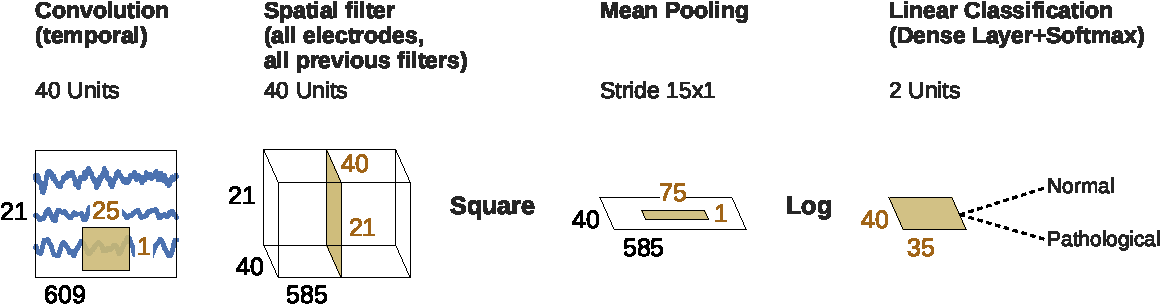
\includegraphics[width=\textwidth]{ShallowNet.pdf}
    \caption{ShallowConvNet结构}
    \label{fig:ShallowConvNet}
\end{figure}

由于EEG原始输入具有时间和通道两个维度的信息,可以被视为具有空间信息的图像数据,因此,论文参考以下几种计算机视觉领域的经典模型,用于网络的特征提取基础结构:

(1) Inception网络

Inception模块起源于经典的GoogLeNet模型\cite{szegedy2015going},并在计算机视觉图像分类任务中取得了优异的效果。传统卷积神经网络倾向于通过加深和拓宽网络结构以增进性能,然而这种做法伴随着参数数量的激增,不仅加大了计算负担,还可能导致过拟合问题。在这种背景下,Inception模块提出了多尺度特征并行抽取的策略,旨在保持网络稀疏性的同时,充分利用密集矩阵运算的高性能。典型的Inception-V1模块的结构如图~\ref{fig:Inception}~所示,其将不同大小的卷积层和最大池化层并行排列,并行地对输入数据执行多种卷积和池化运算,继而将提取到的不同尺度特征在深度维度上进行拼接。这种设计能够在单层网络内并行地提取输入数据在不同层次和粒度的特征信息,从而在高效扩展网络的深度和宽度的同时,有效削减参数规模,提升计算速度。此外,Inception模块中引入了1\times1卷积核,用以实现深度上的特征转化和降维,这种方式能够让模型学习到更为丰富的特征,同时降低计算成本。后续的论文中,Inception模块不断迭代优化,陆续引入了批归一化、深度可分离卷积、矩阵因子分解等技术,进一步提升了模型的性能\cite{szegedy2016rethinking}\cite{szegedy2017inception}。
\begin{figure}
  \centering
  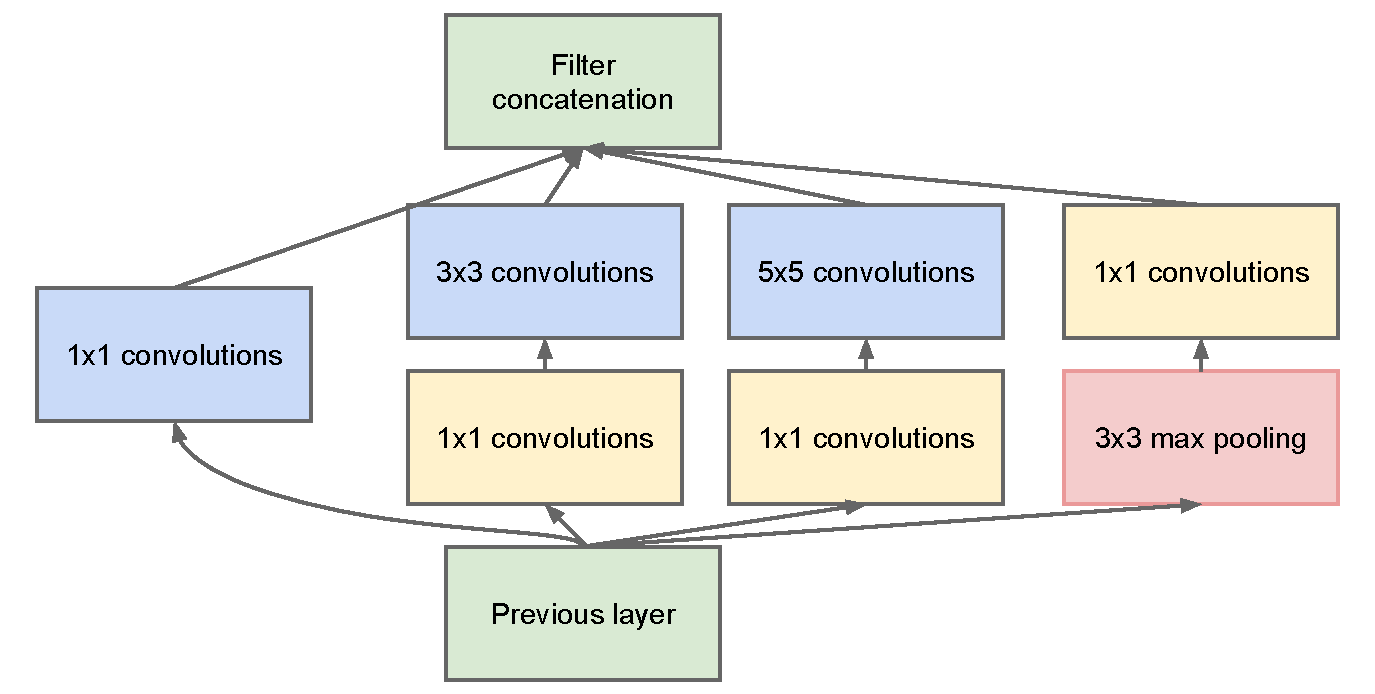
\includegraphics[width=\textwidth]{Inception.pdf}
  \caption{Inception结构}
  \label{fig:Inception}
\end{figure}

(2) 残差神经网络

残差神经网络(Residual Network,ResNet)\cite{he2016deep}是计算机视觉图像识别领域的一个经典模型。ResNet研究发现了深度神经网络的退化现象(Degradation),即随着网络深度不断增加,模型准确率起初随深度上升,却在达到峰值后急剧下滑。针对这种现象,ResNet提出了残差学习框架,其核心思想是引入残差块(Residual Block),每个残差块通过快捷连接(Shortcut Connection)将输入信息直接输送至输出层,使得网络只需要专注学习输入与输出之间的残差信息,而非完整的映射关系。基础的ResNet由一系列残差块堆叠而成,残差块的结构如图~\ref{fig:ResNet}~所示。通过快捷连接,ResNet在训练过程中,梯度能够从深层网络直接回传至浅层,避免网络深度增加带来的训练困难和性能下降问题,从而提升深度神经网络的性能表现和训练效率。
\begin{figure}
  \centering
  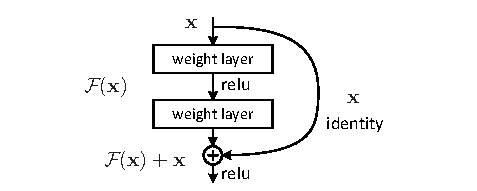
\includegraphics[width=\textwidth]{ResNet.pdf}
  \caption{残差块结构}
  \label{fig:ResNet}
\end{figure}

(3) U-Net

U-Net模型\cite{ronneberger2015u}最初是为生物医学图像分割任务而设计,其具有优秀的性能,尤其在细胞、器官和病变区域的精确标注上表现出色,是医学图像分割领域的主流模型之一。U-Net的独特之处在于其采用了对称的编码-解码结构(Encoder-Decoder)和跳跃连接(skip connection),其结构如图~\ref{fig:UNet}~所示。编码器通过连续的卷积和下采样层对输入图像进行深度特征提取和空间压缩,提炼出高级抽象特征;解码器部分则通过上采样和卷积恢复到与输入图像相同的空间分辨率,同时保留详细的定位信息。跳跃连接将编码器各阶段的特征图直接传递给相应的解码器阶段,有效地结合了包含更多细节信息的浅层特征和包含更多高级语义信息的深层特征,从而在图像分割任务中能够取得更为精细的分割效果。同时,U-Net模型结构简单,易于训练,能够缓解小样本数据集上的过拟合问题。
\begin{figure}
  \centering
  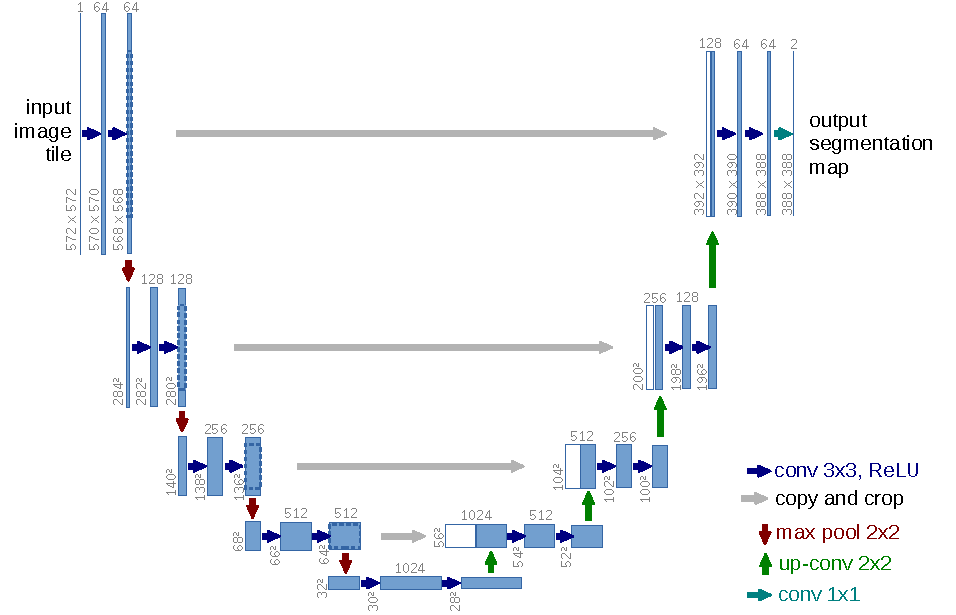
\includegraphics[width=\textwidth]{UNet.pdf}
  \caption{U-Net结构}
  \label{fig:UNet}
\end{figure}

在这三种模型中,Inception和ResNet均在图像分类任务中展现出了优秀的性能。Inception通过同一层网络内的多尺度特征并行抽取,在不显著增加网络深度的前提下,实现了特征提取的广度与效率的提升。ResNet通过引入快捷连接,解决了深度神经网络训练过程中的梯度消失和退化问题,增强了深层次网络的训练效率和性能表现。U-Net则在生物医学图像分割领域取得了优秀的表现,医学图像的语义信息较为简单,且结构较为固定,因此高级语义信息和低级特征都相对重要,U-Net通过跳跃连接保留并融合了这两类信息,同时,U-Net参数量较小,不容易在小样本数据集上发生过拟合现象。论文选择将U-Net迁移至MI-EEG分类任务中,是因为EEG信号具有与生物医学图像类似的生理特性,如特征相对简单、数据集规模偏小等。

为了验证Inception、ResNet与U-Net在EEG信号分类任务中的性能,论文在BCI Competition IV Dataset 2A数据集上进行实验对比。在实验设置中,统一将三种模型的网络深度调整为三层,并对其他关键参数如卷积核大小、学习率等进行了固定,此外,对这三种模型的原始代码进行了调整,使得其适应MI-EEG分类任务。实验结果如表~\ref{tab:Incep-Res-U}~所示,主要展示准确率(Accuracy,ACC)和Kappa一致性系数(Kappa)指标,这两项指标是数据集中九位受试者的平均表现。
\begin{table}[ht]
  \centering
  \caption{Inception、ResNet、U-Net实验结果对比}
  \label{tab:Incep-Res-U}
  \begin{tabularx}{\textwidth}{CCC}
    \toprule
    Models & ACC(\%) & Kappa \\
    \midrule
    Inception & \textbf{67.40} & \textbf{0.56} \\
    ResNet & 56.94 & 0.43 \\
    U-Net & 62.27 & 0.50 \\
    \bottomrule
  \end{tabularx}
\end{table}

实验数据显示,Inception模型在这三种模型中具有最优的性能表现,U-Net次之,ResNet的表现则相对较差。这可能是因为同样的网络深度下,Inception模型得益于多尺度并行特征提取机制,能更全面地捕获EEG信号的多种特征。相比之下,U-Net虽然通过跳跃连接有效地结合了EEG信号的低层特征和高层语义信息,但在解码器阶段,U-Net将特征图重建至原始空间尺寸的过程可能为分类任务引入了不必要的复杂性。ResNet的快捷连接在较浅层网络结构中可能未能完全发挥其优势,更适用于深层次网络。实验结果与过往研究中关于浅层网络更适合MI-EEG分类任务的研究结论相互印证。综上所述,论文选用Inception模块作为MI-EEG信号特征提取的基础结构,旨在保持模型简洁高效的同时,在MI-EEG分类任务中取得更好的性能。

EEG信号的空间特征复杂度通常低于时间特征复杂度,时空信息具有不均衡性。例如,在BCI Competition IV Dataset 2B\cite{tangermann2012review}数据集中,仅仅使用了三个电极采集MI-EEG信号,使得空间信息相对时间信息更为稀疏。因此,论文采取更关注时间特征的策略,即将Inception模块应用于时间卷积层中,使得时间卷积层的复杂度要高于空间卷积层的复杂度,这一策略的目的在于使得模型具有捕捉高维时空特征能力的同时,防止模型因复杂度过高而在小样本数据集上过早地发生过拟合现象。

空间卷积层有两种不同的方式融入基于Inception改进的时间卷积层之后,一种是在每个Inception模块内部的分支结构上增加空间卷积层,另一种则是在整个Inception模块之后附加空间卷积层。图~\ref{fig:ts-incep}~展示了这两种引入方式的区别,将这两种方式分别称为分支内融合(Inception-In)和模块后融合(Inception-After),需要说明的是,图中省略了网络的其他结构,如瓶颈层等,以尽可能简洁地展现不同引入方式的差异。
\begin{figure}
  \centering
  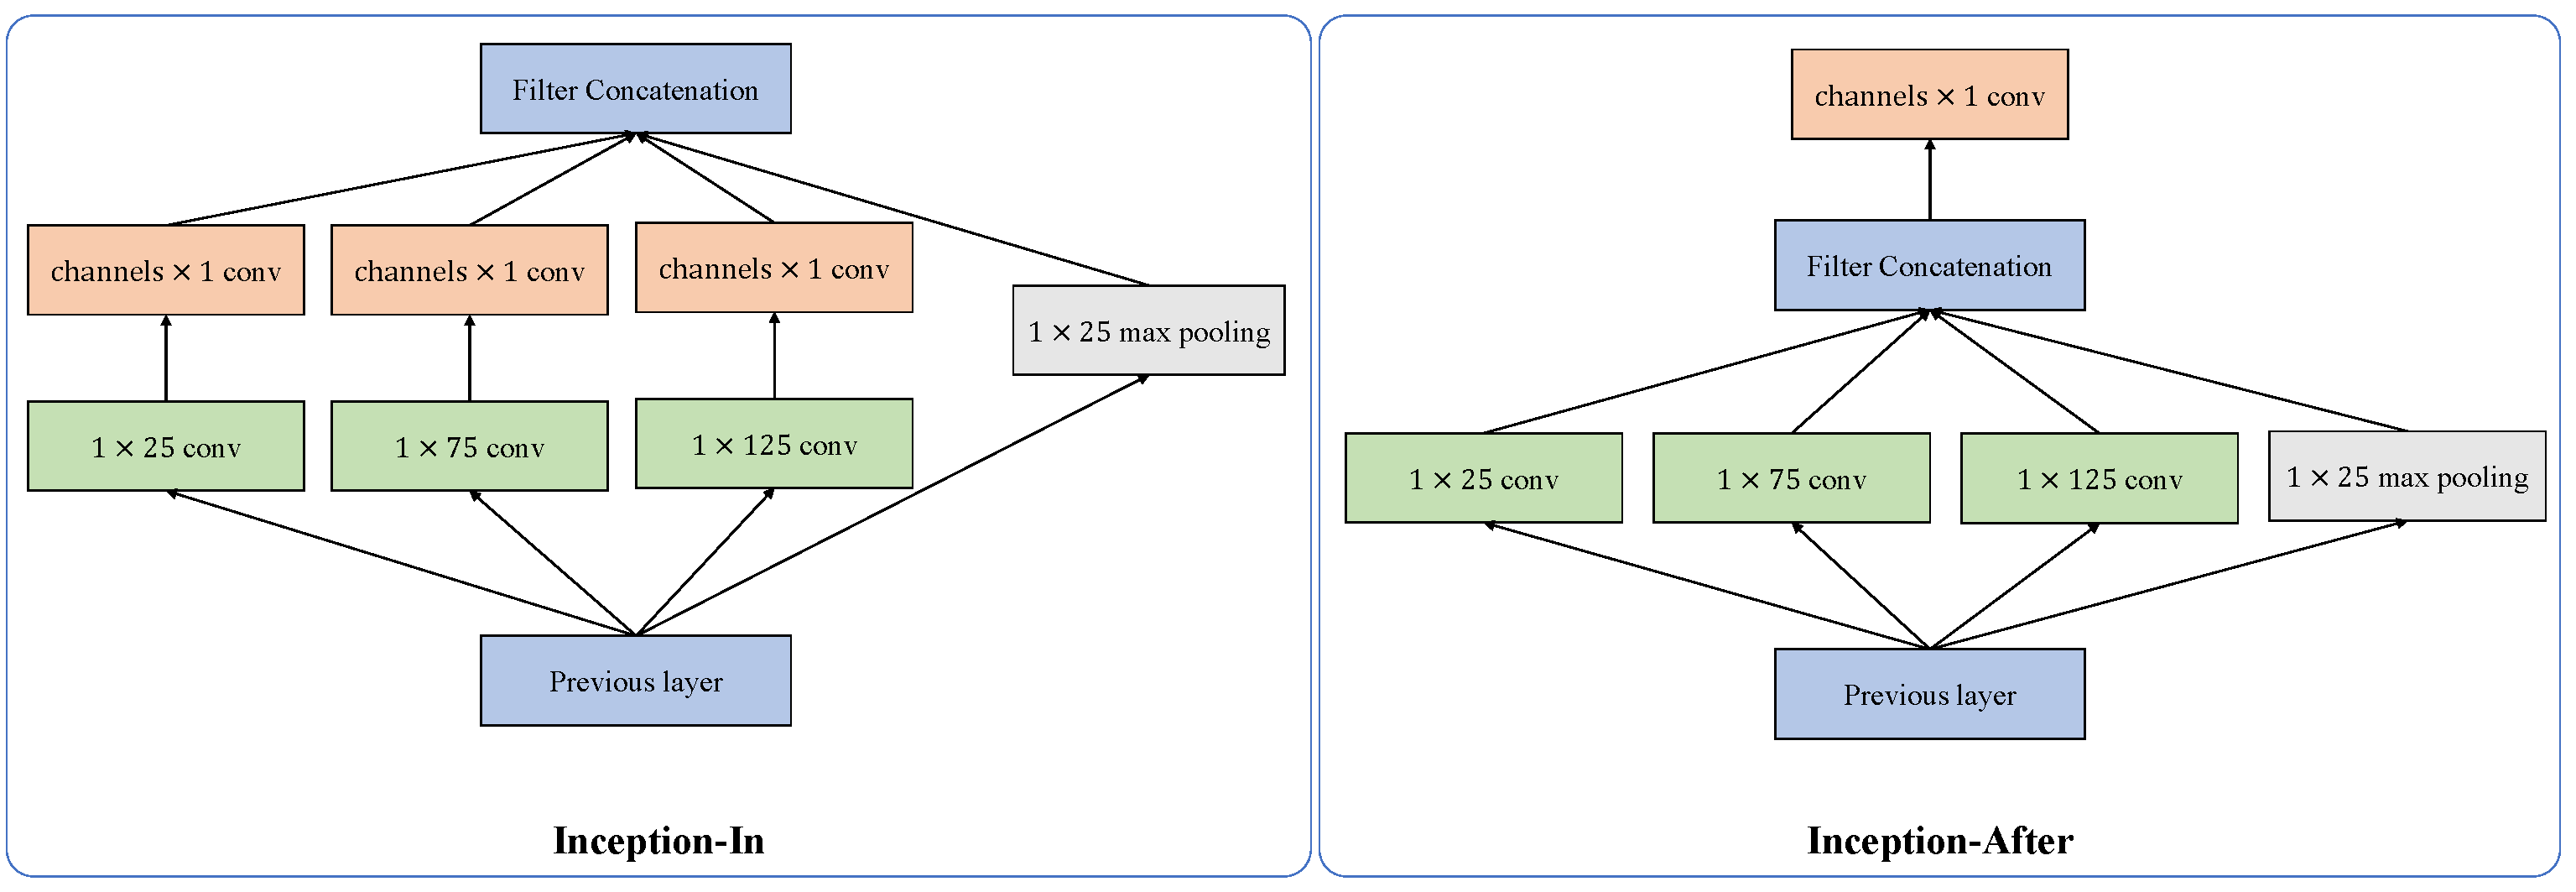
\includegraphics[width=\textwidth]{ts-incepv2.pdf}
  \caption{Inception模块引入空间卷积层的方式}
  \label{fig:ts-incep}
\end{figure}

为了比较Inception-In与Inception-After的性能差异,论文在BCI Competition IV Dataset 2A数据集上设计实验进行对比。在实验设置阶段,固定了Inception模块的层次数量、分支数量等参数,实验结果如表~\ref{tab:ts-inception}~所示。在此,重点关注两项评价指标——准确率(Accuracy, ACC)和Kappa一致性系数(Kappa),这两项指标均基于数据集中九位受试者的平均表现。实验结果显示,Inception-After方式在准确率和一致性系数上均表现更优。这一优势可能源自两方面的原因:一方面,虽然Inception-In模式借鉴了FBCSP算法的分频段处理思路,但在Inception分支内部直接进行空间特征提取的过程中,损失了部分空间全局信息;另一方面,Inception-In结构具有相对更大的参数规模,这可能导致模型在有限样本条件下更容易出现过拟合现象。基于以上分析和实验验证,论文选择以Inception-After的方式布局时间卷积层与空间卷积层。
\begin{table}[ht]
  \centering
  \caption{Inception-In、Inception-After实验结果对比}
  \label{tab:ts-inception}
  \begin{tabularx}{\textwidth}{CCC}
    \toprule
    Models & ACC(\%) & Kappa \\
    \midrule
    Inception-In & 63.31 & 0.51 \\
    Inception-After & \textbf{75.35} & \textbf{0.70} \\
    \bottomrule
  \end{tabularx}
\end{table}

文献\cite{lawhern2018eegnet}\cite{schirrmeister2017deep}指出,在EEG信号解码任务中,增加神经网络的深度有利于提升解码精度。瓶颈层(Bottleneck Layer)是深度神经网络中的常见结构\cite{he2016deep}\cite{huang2017densely},通常用于对数据的降维和升维,由于采用了1\times1卷积进行操作,瓶颈层能够有效地减少神经网络的参数。不同于原始Inception模块中通过瓶颈层进行数据降维的操作,论文使用瓶颈层对数据进行升维操作,并将瓶颈层提取至卷积和池化操作之前,其目标为在深度维度上促进时空信息的融合。

为了加快网络训练速度,并避免小数据集下过早的过拟合,论文在引入瓶颈层的基础上,对网络的结构进行了进一步的调整:

(1) 借鉴EEGNet\cite{lawhern2018eegnet}的结构,将时间卷积和空间卷积替换为参数量更少的深度可分离卷积\cite{lawhern2018eegnet};

(2) 在模型中引入了一系列正则化技术,包括批量归一化(Batch Normalization,BN)和随机Dropout等。

此外,论文将ShallowConvNet中的对数激活函数替换为GELU激活函数,前者基于FBCSP算法中的对数方差计算提出,后者基于高斯分布和自然梯度流提出,能够更自然地模拟神经元的概率行为,具有更好的连续性和光滑性\cite{hendrycks2016gaussian},实验证明了GELU激活函数较之对数激活函数具有更好的效果。

论文将改进后得到的基础模型称为BaseNet,其结构如图~\ref{fig:BaseNet}~所示。需要注意的是,Inception模块的层次数量和分支数量是影响其性能表现的两项可调的超参数。
\begin{figure}
    \centering
    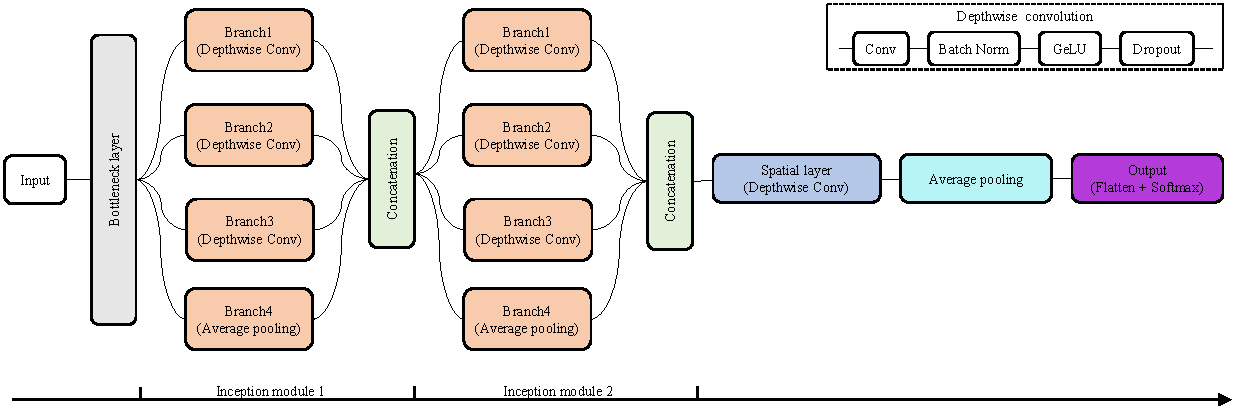
\includegraphics[width=\textwidth]{Base-Net.pdf}
    \caption{BaseNet结构}
    \label{fig:BaseNet}
\end{figure}

\subsection{局部混合注意力svSE}

注意力机制的提出受到人类认知科学的启发,其核心理念在于模拟人类大脑在处理信息过程中的选择性关注机制,即并非均匀地分配注意力处理对待所有输入,而是将注意力主动、动态且有选择性地聚焦于最重要或最相关的信息上。自二十世纪被提出以来\cite{730558},注意力机制在计算机视觉、自然语言处理等领域得到了广泛的应用,并表现出了优秀的效果。根据神经科学先验知识,EEG信号中不同的通道和采样点具有不同的重要性,这为在MI-EEG分类领域应用注意力机制提供了理论依据,此外,将二维EEG信号视为一种由通道和时间两个维度构成的特殊图像,使得在MI-EEG分类领域能够迁移应用计算机视觉领域中的注意力机制。

计算机视觉领域中经常使用的注意力机制有:

(1) 通道注意力机制
    
不同于EEG信号中代表电极的通道,计算机视觉领域的通道代表图像的不同特征映射。通道注意力机制用于调整不同特征通道的重要性,通常会对每一个特征通道计算一些全局统计量,如均值、方差等,再将这些统计量经过非线性变换层进行编码,最后将编码向量进行转换并用于各个特征通道的加权。通道注意力机制的经典模型是压缩和激励网络(Squeeze-and-Excitation Networks,SENet)\cite{8578843},其主要思想即是压缩(Squeeze)和激励(Excitation),SENet首先通过压缩操作获取全局上下文信息,然后通过激励操作对每个通道独立生成权重系数。具体而言,在压缩操作中,SENet在空间维度执行全局池化操作,将每个通道的特征图汇总成一个标量值;然后,在激励操作中,SENet通过一个全连接网络生成每个通道的权重系数,这些权重系数用于重新加权每个通道的特征图,以增强有用的特征并抑制无用的特征。

在后文中,为避免与计算机视觉领域中的概念相混淆,在MI-EEG分类任务中,用深度来代表EEG信号的不同特征映射,而通道仍然代表电极。

(2) 空间注意力机制
    
在计算机视觉领域中,空间注意力机制用于调整图片、视频等输入数据在空间维度中不同区域的重要性,通常会在深度维度上通过全局池化、卷积、特征融合等操作生成一个与特征图尺寸相同的注意力图,其值反映了空间维度中不同区域的注意力强度,最后,将注意力图进行转换,并用于原始特征图的加权。空间注意力机制的经典模型是空间变换网络(Spatial Transformer Network,STN)\cite{jaderberg2015spatial},其具有对输入数据进行空间变换的能力,能够自动捕获重要区域的特征。

(3) 混合注意力机制
    
混合注意力机制是一种集成多种注意力机制(如空间注意力、通道注意力及自注意力等)的方法,旨在更全面地捕获和整合输入数据在不同维度的有效信息。混合注意力机制通常会使用不同的注意力机制分别计算原始特征图的注意力权重,再将这些注意力权重进行融合,最后将融合后的注意力权重用于原始特征图的加权,或者将不同的注意力权重用于原始特征图加权,再将加权特征图进行融合。混合注意力机制的经典模型有卷积注意力机制模块(Convolutional Block Attention Module,CBAM)\cite{woo2018cbam}、空间与通道压缩与激励模块(Spatial and Channel Squeeze-and-Excitation,scSE)\cite{roy2018concurrent}等。
    
CBAM结合了通道注意力机制与空间注意力机制,其结构如图~\ref{fig:CBAM}~所示,输入特征图首先经过通道注意力模块进行加权,再通过空间注意力模块进行加权,从而得到最终结果。
\begin{figure}
    \centering
    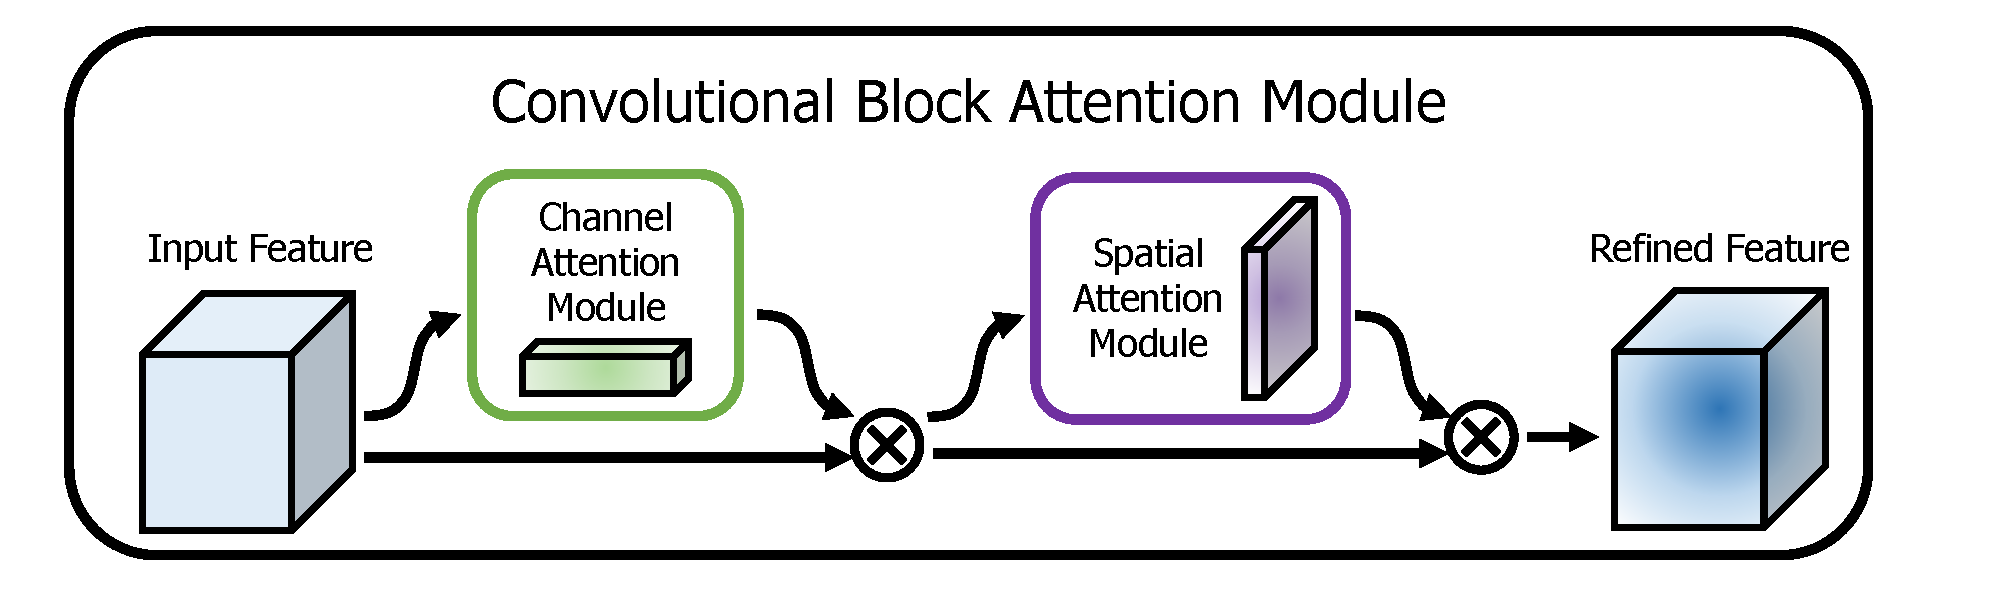
\includegraphics[width=\textwidth]{CBAM.pdf}
    \caption{CBAM结构}
    \label{fig:CBAM}
\end{figure}

具体而言,在通道注意力模块中,输入特征图分别进行空间维度上的全局最大池化和全局平均池化,再将得到的统计值分别通过一个共享权重的全连接层,最后经过逐点加和与非线性变换得到通道注意力权重,用于输入特征图的加权。空间注意力模块的输入是经过通道注意力加权的特征图,首先在通道维度上进行全局最大池化和平均池化,再将得到的统计值在通道维度进行拼接,最后经过卷积降维与非线性变换得到空间注意力权重,与特征图加权后得到最终结果。CBAM的模块结构如图~\ref{fig:CBAM-Block}~所示。
\begin{figure}
  \centering
  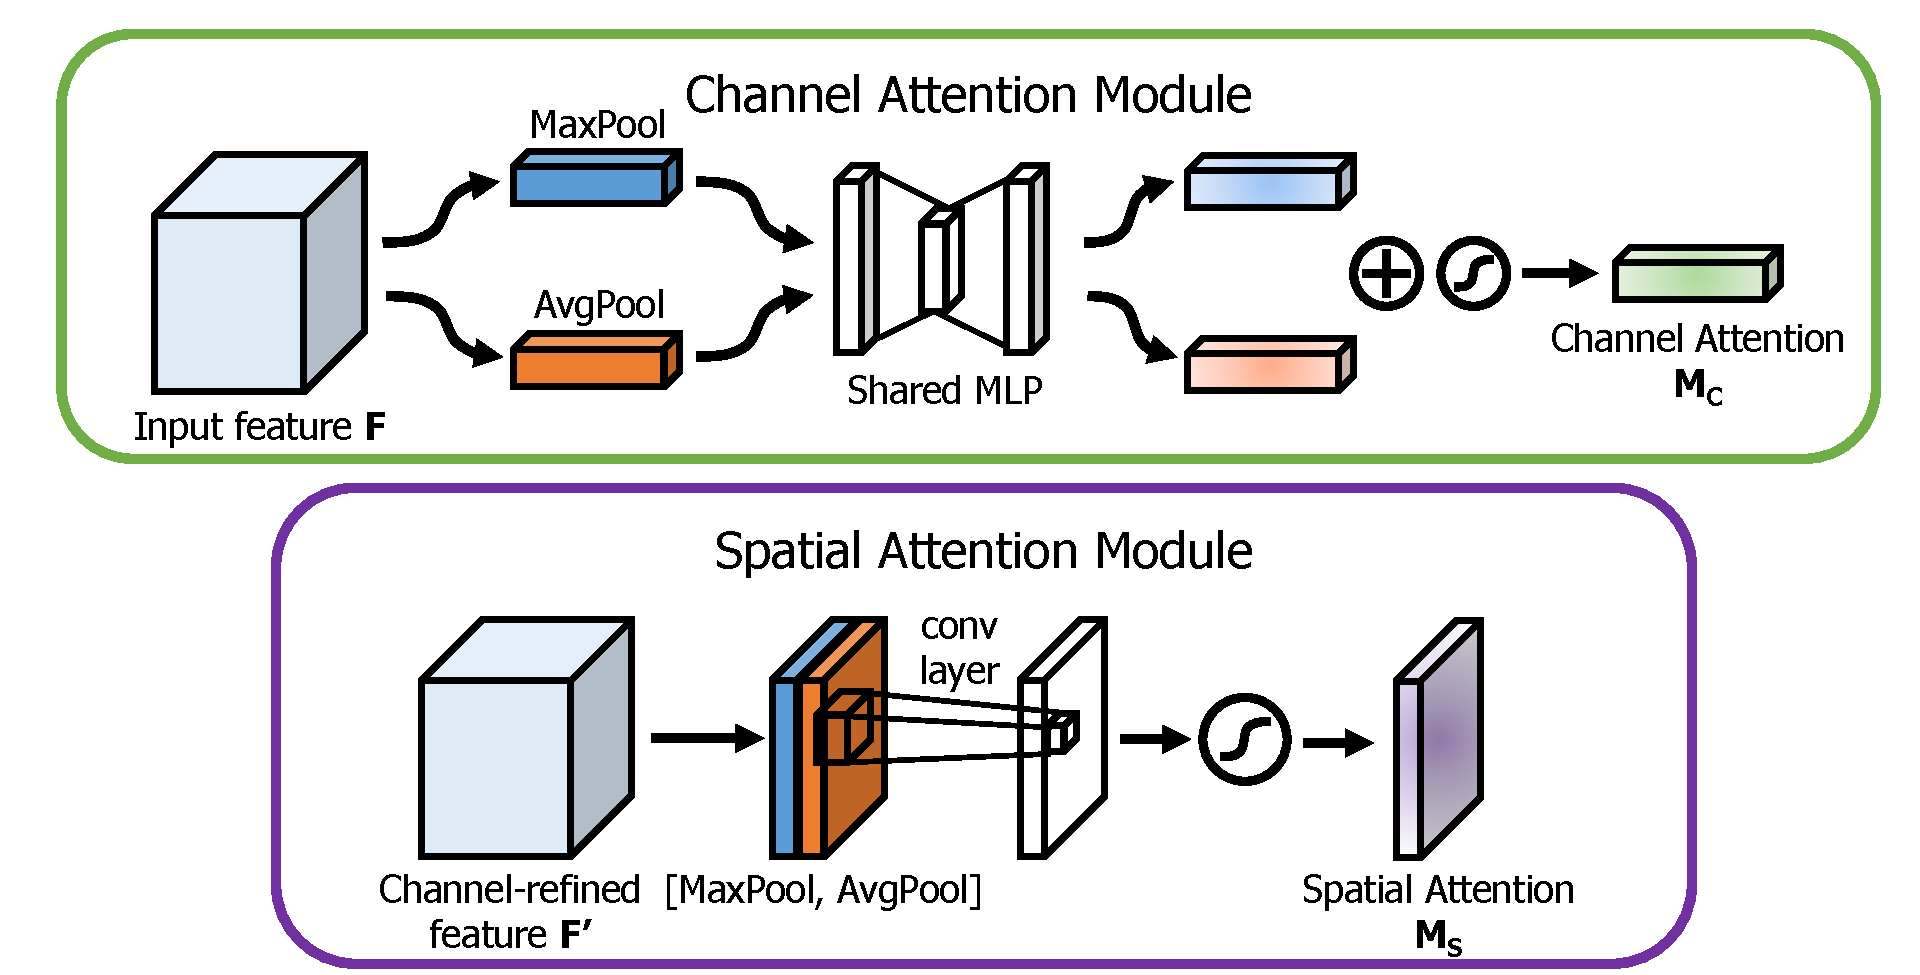
\includegraphics[width=\textwidth]{CBAM-Block.pdf}
  \caption{CBAM模块结构}
  \label{fig:CBAM-Block}
\end{figure}

scSE同样结合了通道注意力机制与空间注意力机制,基于SENet提出了一种通道注意力模块(Channel Squeeze-and-Excitation,cSE)和一种空间注意力模块(Spatial Squeeze-and-Excitation,sSE),其结构如图~\ref{fig:scSE}~所示,不同于CBAM,scSE的两个子模块并行处理原始输入,分别在空间维度和通道维度对原始输入进行加权,最后再进行特征图的融合。具体而言,cSE模块中,原始输入依次经过了空间维度的全局平均池化,通道维度的卷积降维与升维,以及非线性变换,以得到通道注意力权重。sSE模块中,直接通过深度卷积在通道维度进行降维,再经过非线性变换以得到空间注意力权重。
\begin{figure}
    \centering
    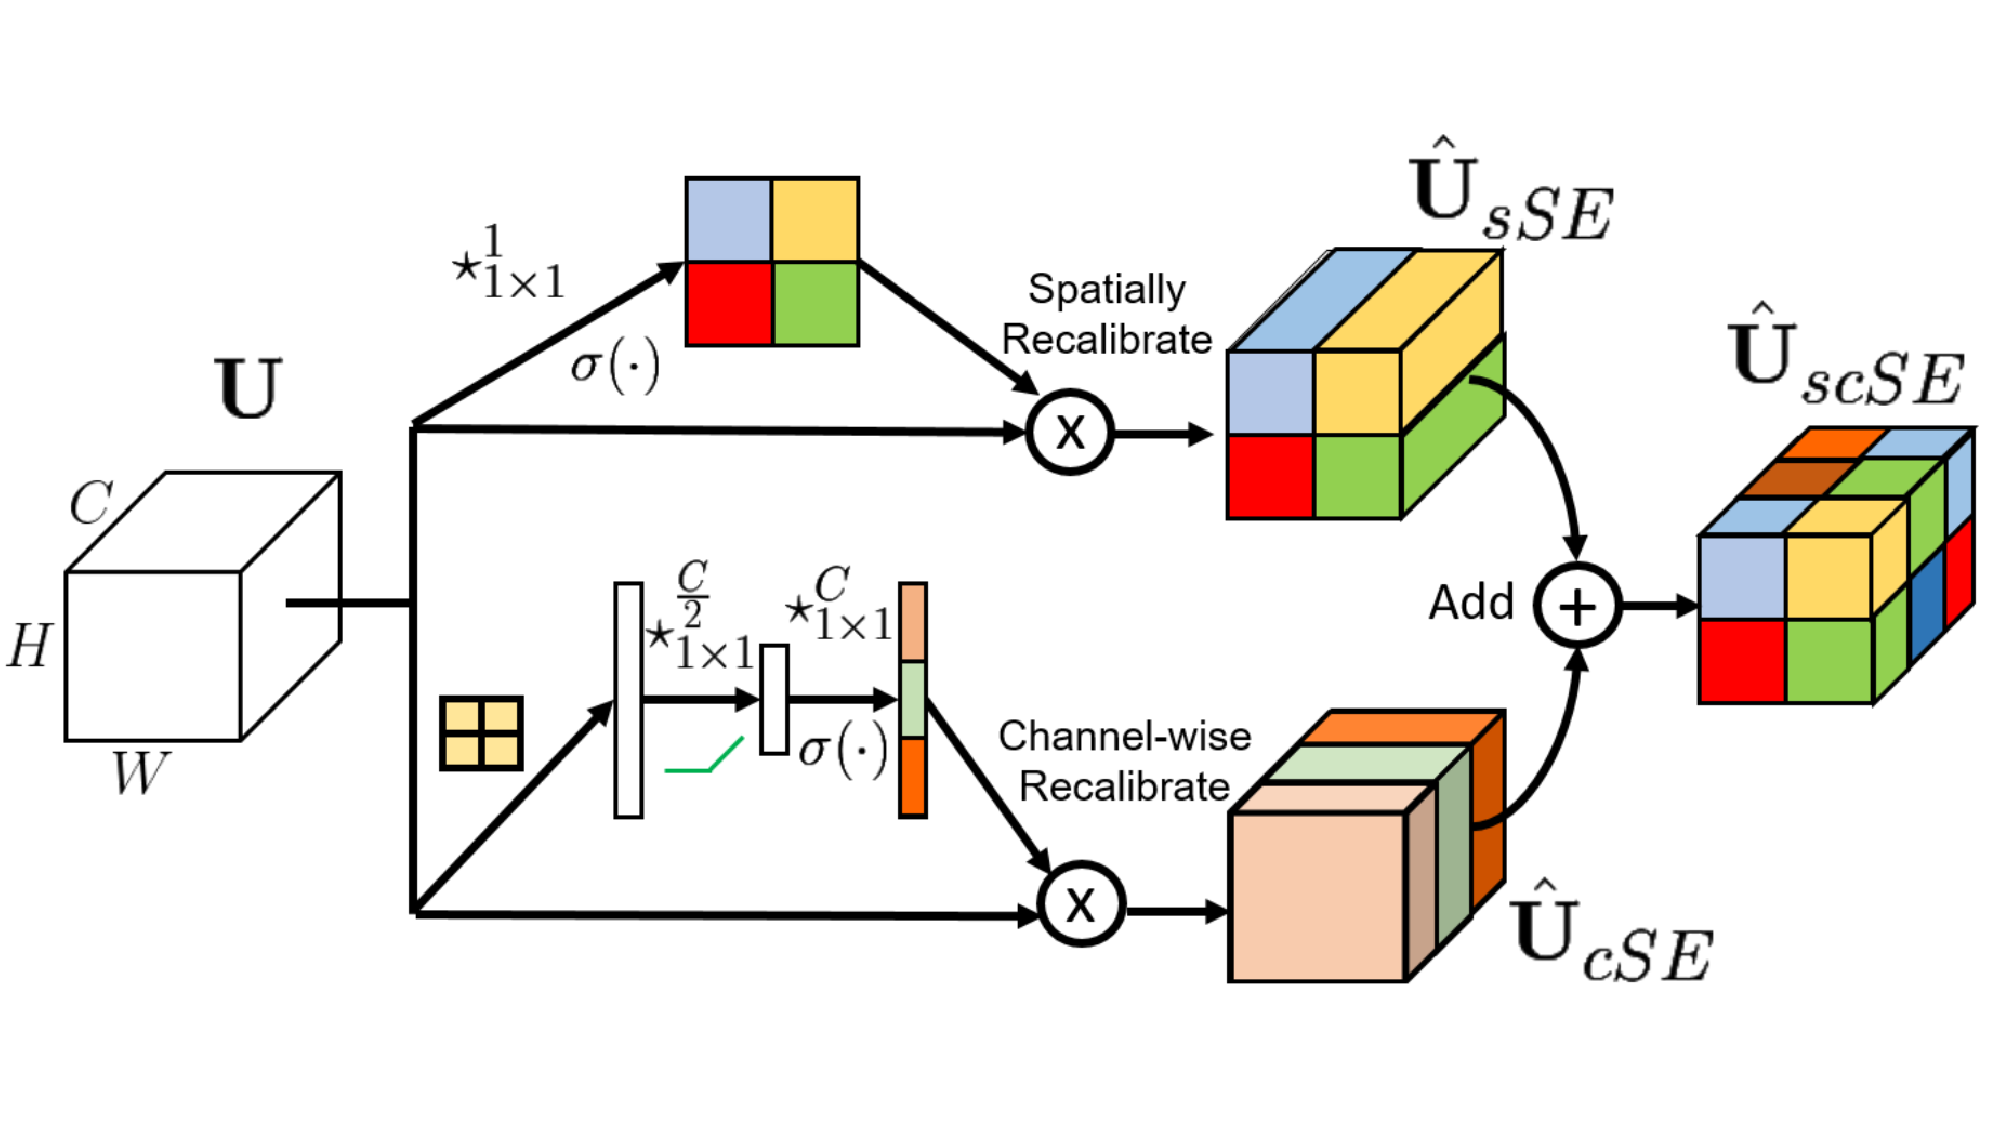
\includegraphics[width=\textwidth]{scSE.pdf}
    \caption{scSE结构}
    \label{fig:scSE}
\end{figure}

注意力机制通过动态分配权重,使得模型能够聚焦于输入数据中的关键信息,削弱噪声的影响,混合注意力机制则结合了多种注意力机制的优点,从而能够更全面地捕获和整合不同维度的数据特征,并在许多情况下展现出优于单一注意力机制的性能。因此,论文将升维处理后的EEG信号视作具有深度信息的图像数据,采用结合了深度注意力和空间注意力的混合注意力机制对BaseNet进行改进。

CBAM模块和scSE模块均为轻量级注意力模块,且均兼顾深度注意力和空间注意力,但scSE模块在参数数量上更具优势。与此同时,文献\cite{roy2018concurrent}研究发现scSE模块在语义分割任务上表现出色,特别是在与EEG信号拥有相似生理特性的医学图像的分割任务,其性能优于CBAM模块。基于以上理由,论文选择将scSE模块引入BaseNet模型中。由于BaseNet的特征提取过程分为时间卷积和空间卷积两个阶段,scSE模块可采取以下三种引入方式:其一是在时间卷积层后引入;其二是在空间卷积层后引入;其三是同时在时间卷积层和空间卷积层之后引入。图~\ref{fig:att-Base}~展示了这三种引入scSE模块的方式,从左至右分别是时间卷积层后引入scSE模块、空间卷积层后引入scSE模块,以及在时间卷积和空间卷积层后均引入scSE模块。将这三种引入方式对应的模型分别简称为S-Temporal-BaseNet、S-Spatial-BaseNet、S-TS-BaseNet。
\begin{figure}
  \centering
  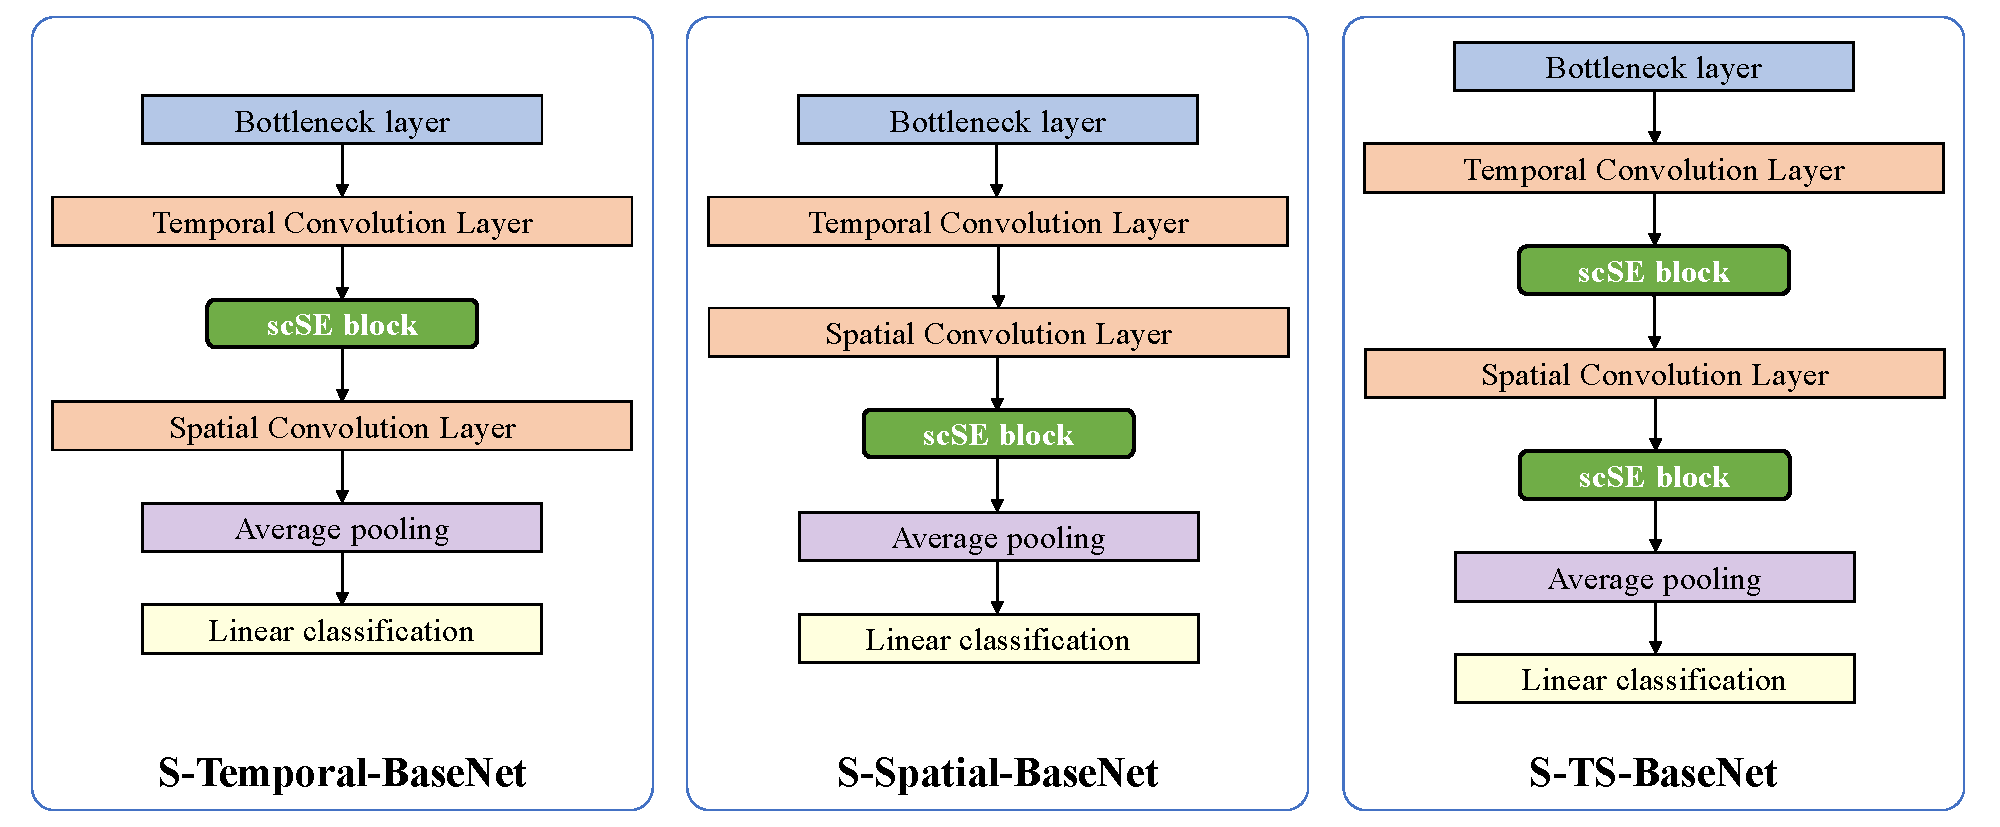
\includegraphics[width=\textwidth]{att-Base.pdf}
  \caption{BaseNet引入注意力模块的方式}
  \label{fig:att-Base}
\end{figure}

表~\ref{tab:scSE-BaseNet}~展示了S-Temporal-BaseNet、S-Spatial-BaseNet、S-TS-BaseNet三种模型在BCI Competition IV Dataset 2A\cite{tangermann2012review}数据集上的对比实验结果。实验采用固定的参数,表格中展示的准确率(Accuracy,ACC)和Kappa一致性系数(Kappa)指标为数据集中九位受试者的平均表现,标准差(Standard Deviation,SD)则为准确率的标准差。从准确率和一致性分析,S-ST-BaseNet模型的效果优于其他两种模型,与经验相符。此外,S-Temporal-BaseNet模型的效果优于S-Spatial-BaseNet模型,其原因可能在于,空间卷积层沿通道维度的卷积和沿深度维度的降维使得数据损失了部分特征,进而减弱了scSE模块提取关键特征权重的能力,而时间卷积层保留了大部分深度信息和通道信息,因此,在时间卷积层之后加入scSE模块能够帮助模型更好地捕捉深度和空间的特征。从标准差分析,S-TS-BaseNet模型的准确率波动幅度较小,对不同受试者的MI-EEG分类效果相对均衡,另外两种模型在不同受试者间的分类精度则存在较为明显的差异。实验数据显示,S-TS-BaseNet模型在增加了少量参数的情况下,取得了更好的效果,因此,论文采用同时在时间卷积层和空间卷积层之后引入scSE模块的方式,将这种结构的模型称为S-BaseNet。
\begin{table}[ht]
  \centering
  \caption{scSE模块引入位置对比}
  \label{tab:scSE-BaseNet}
  \begin{tabularx}{\textwidth}{CCCCC}
    \toprule
    \makebox[0.2\textwidth][c]{Models} & \makebox[0.2\textwidth][c]{ACC(\%)} & \makebox[0.2\textwidth][c]{Kappa} & \makebox[0.2\textwidth][c]{SD} & \makebox[0.2\textwidth][c]{Parameters} \\
    % Models & ACC(\%) & Kappa & SD & Parameters \\
    \midrule
    \makebox[0.2\textwidth][c]{S-Temporal-BaseNet} & \makebox[0.2\textwidth][c]{78.09} & \makebox[0.2\textwidth][c]{0.71} & \makebox[0.2\textwidth][c]{10.38} & \makebox[0.2\textwidth][c]{4702} \\
    \makebox[0.2\textwidth][c]{S-Spatial-BaseNet} & \makebox[0.2\textwidth][c]{77.16} & \makebox[0.2\textwidth][c]{0.69} & \makebox[0.2\textwidth][c]{10.24} & \makebox[0.2\textwidth][c]{\textbf{4357}} \\
    \makebox[0.2\textwidth][c]{S-TS-BaseNet} & \makebox[0.2\textwidth][c]{\textbf{78.55}} & \makebox[0.2\textwidth][c]{\textbf{0.71}} & \makebox[0.2\textwidth][c]{\textbf{9.46}} & \makebox[0.2\textwidth][c]{4765} \\
    \bottomrule
  \end{tabularx}
\end{table}

为取得更好的效果,对scSE模块进行改进。针对cSE模块,采用全局最大池化取代全局平均池化操作,实验证明了这一改动使模型具有更好的效果。此外,将scSE模块中的Sigmoid激活函数替换为Softmax激活函数,旨在更好地利用全局信息。针对sSE模块,论文提出两种方式进行改进,并将两种方式所得的权重相结合以获取最终的输出:

(1) 由CBAM模块的多维全局池化思想以及FBCNet模型的方差层设计\cite{mane2021fbcnet}得到启发,采用深度维度上的全局平均池化和全局方差计算操作代替原模块中的压缩操作,随后通过深度卷积对深度维度的特征图进行聚合,在更好地表征EEG信号特性的同时,进一步降低了参数规模;

(2) 考虑EEG信号中的时空权重无关性,即空间特征权重代表电极重要程度,时间特征权重代表采样点重要程度,分两个维度提取特征。对于空间维度,首先进行深度压缩操作,随后通过时间维度上的平均池化和最大池化得到两个特征图,通过1\times1卷积对这两个特征图进行融合。对于时间维度,进行空间维度上的卷积操作,以得到时序权重。最后,将空间权重与时序权重相乘,恢复维度。

得到论文将改良后的scSE模块称为svSE(Separate Variance-Informed Spatial and Channel Squeeze-and-Excitation)模块,其结构如图~\ref{fig:svSE}~所示。使用svSE模块替换S-BaseNet模型中的scSE模块。
\begin{figure}
  \centering
  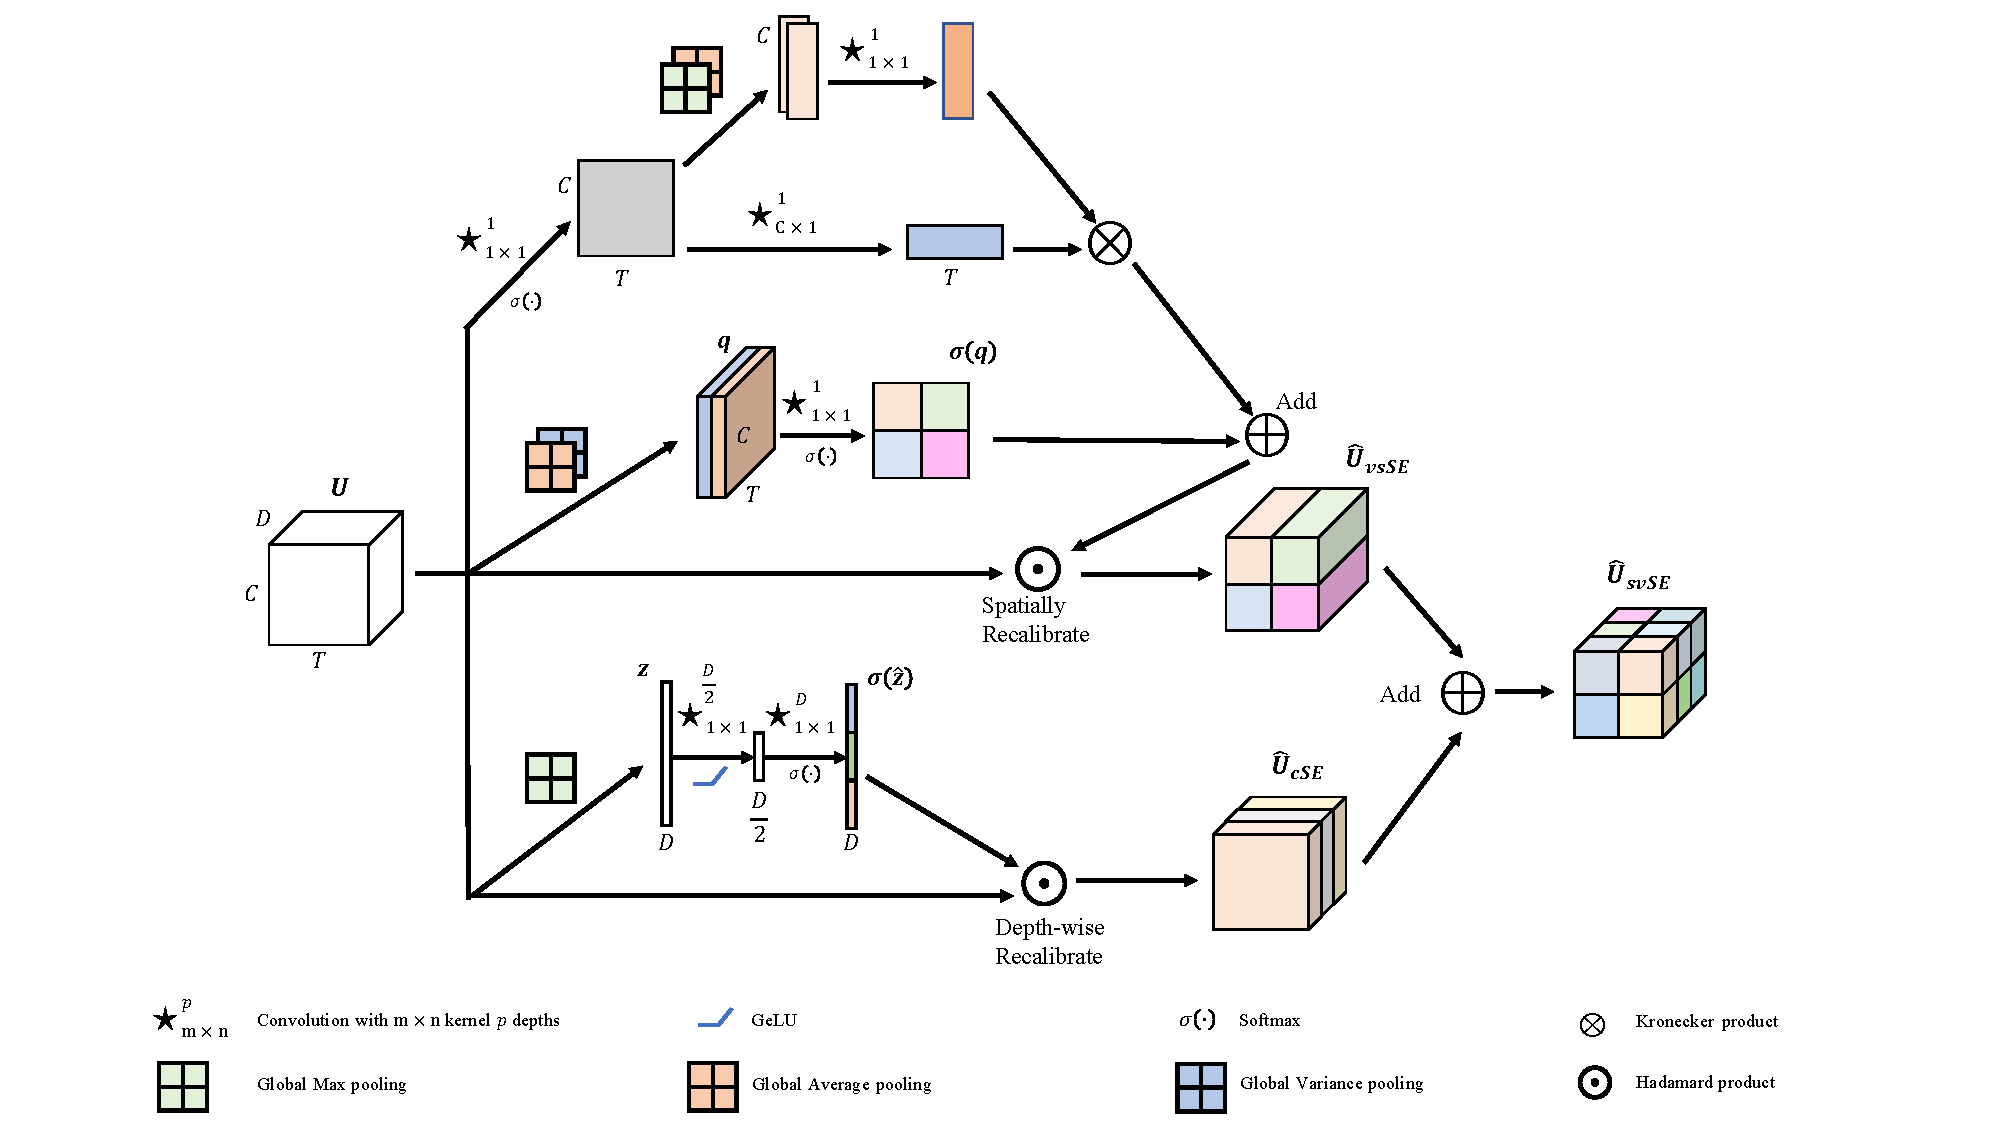
\includegraphics[width=\textwidth]{svSE.pdf}
  \caption{svSE结构}
  \label{fig:svSE}
\end{figure}

\subsection{基于密集连接优化Inception模块}

在构建BaseNet时,论文发现U-Net在处理MI-EEG分类任务时同样展现了一定的优势。由于EEG信号的特征相对简单,因此低级特征与高级语义信息都相对重要,U-Net因其特殊的跳跃连接结构有效地融合了这两种信息,然而,U-Net中通过解码器阶段将特征图恢复至原始空间尺寸的操作并非必要,因为在分类任务中,这种重建过程可能导致额外的计算负担且对分类性能的提升效果不明显。因此,在对VSNet进行改进时,论文从U-Net兼顾低级特征与高级语义信息的策略中得到启发,同时对不必要的特征图空间尺寸还原过程进行规避,以构建一个既能充分利用EEG信号中各级别特征信息,又具备高效计算能力的改进模型。

Gao Huang等人于2016年提出了密集连接网络\cite{huang2017densely}(Dense Convolutional Network,DenseNet)。在ResNet的基础上,DenseNet提出了一种更为激进的连接模式:引入从任意层到后续层的直接连接,即密集连接(Dense Connection)。DenseNet的第 \(l\) 层接收所有前序特征图为输入,其输出为 \(x_l\):
\begin{equation}
  x_l = H_l([x_0, x_1, ···, x_{l-1}])
  \label{eq:dense-conn}
\end{equation}
其中,\([x_0, x_1, ···, x_{l-1}]\) 代表第 \(0, ···, l-1\) 层的输出特征图,\(H_l(·)\) 代表非线性转换复合函数,可能包括一系列的批量归一化、ReLU、池化及卷积操作。密集连接的结构如图~\ref{fig:denseBlock}~所示。
\begin{figure}
  \centering
  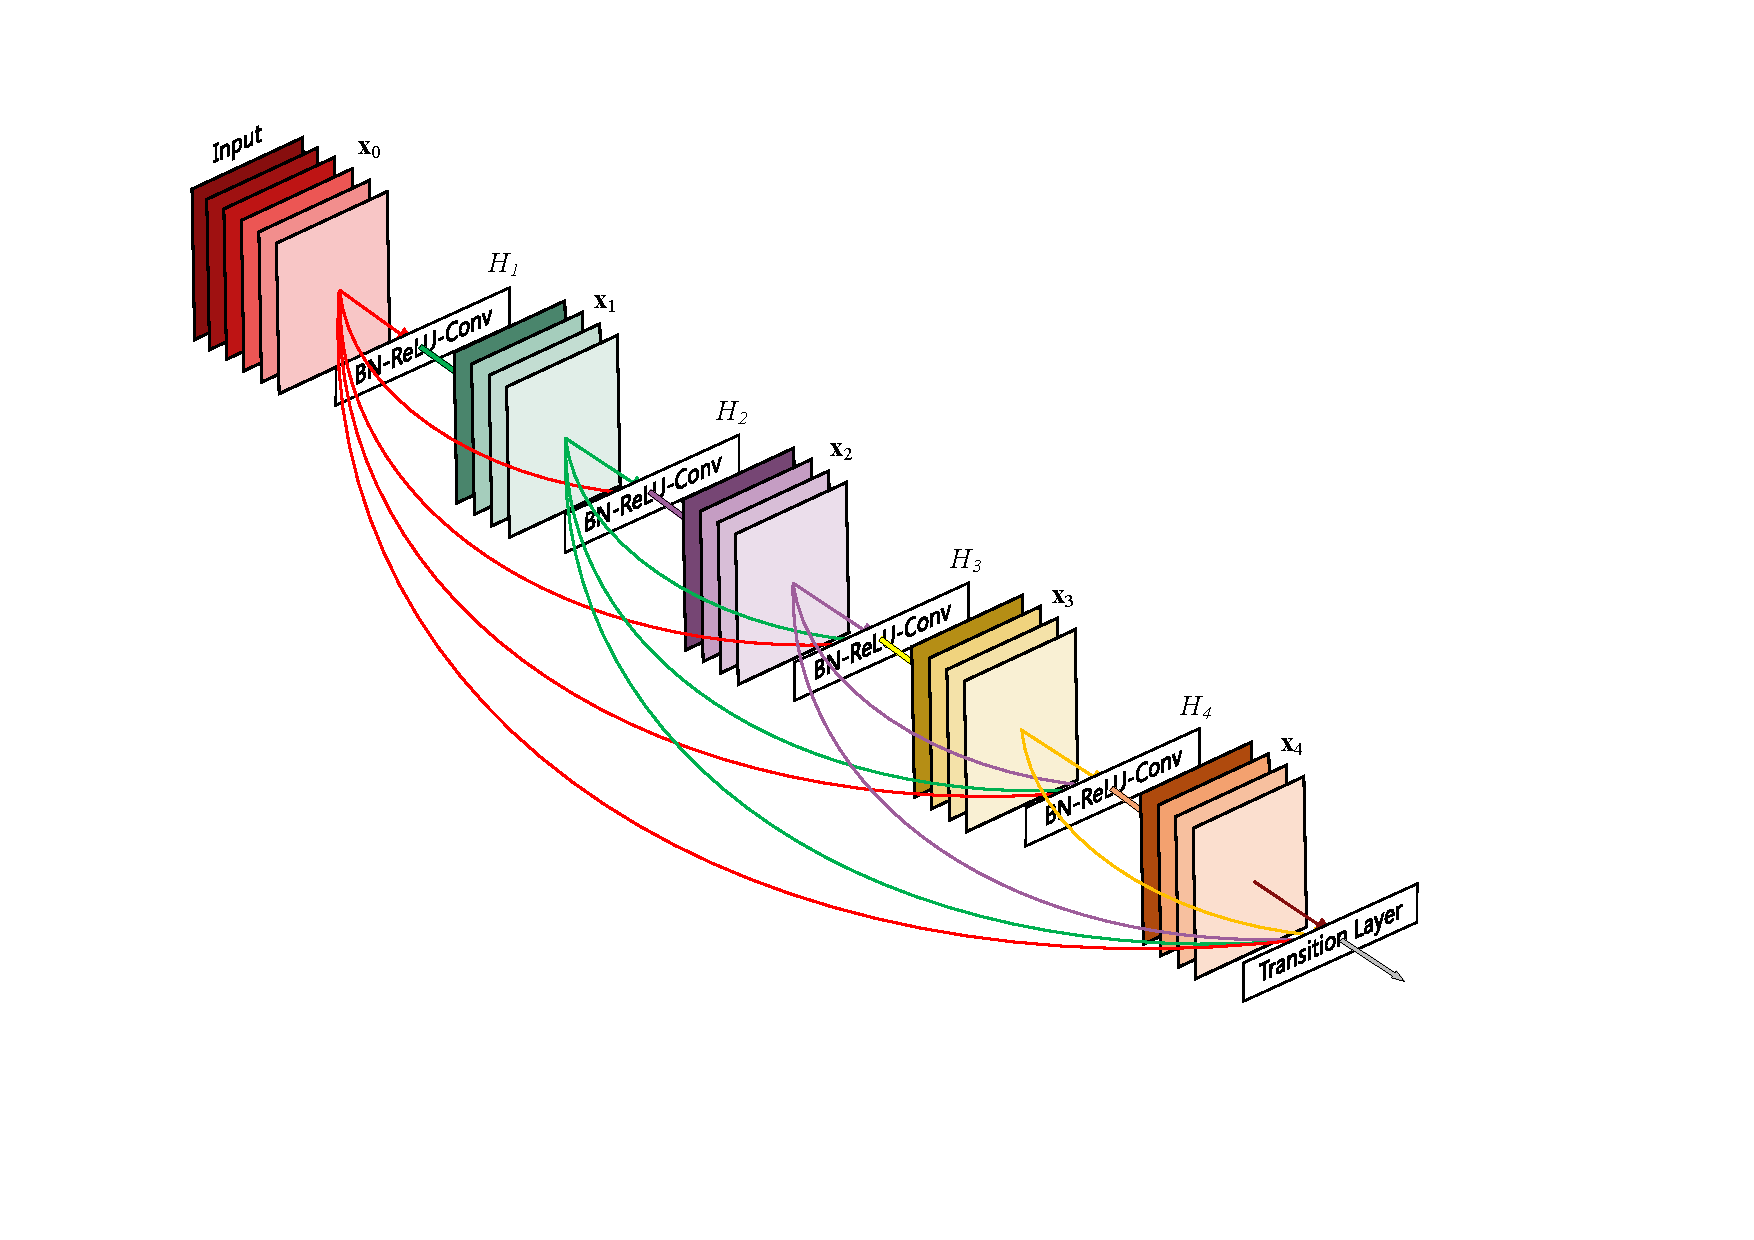
\includegraphics[width=0.8\textwidth]{denseBlock.pdf}
  \caption{密集连接结构}
  \label{fig:denseBlock}
\end{figure}

在密集连接模块中,所有的前序特征图通过Concentrate在深度维度上连接在一起,因此,在一个密集连接模块中所有特征图的大小是相同的。DenseNet提出了Transition模块用于连接两个相邻的密集连接模块,并通过池化操作对特征图进行下采样,从而减小特征图的大小。

通过密集连接的方式,网络中的每一层都能够访问并整合所有前序层提取出的特征信息,进而充分利用EEG信号中的低层特征细节和高层语义信息。相较于U-Net中的编码-解码结构,密集连接无需经历数据空间的重建过程,即可实现特征的有效复用。此外,DenseNet中的Transition模块也为实现特征图的下采样提供了思路。

在DenseNet中,有两种不同构造的密集连接模块,分别是基础密集连接模块(Basic Dense Block)和带有瓶颈层的密集连接模块(Bottleneck Dense Block),它们的区别主要体现在非线性转换复合函数 \(H(·)\) 的设计上:

(1) 基础密集连接模块(Basic Dense Block):其非线性转换复合函数定义为: \(H(·) = BN + ReLU + 3 \times 3\;conv\)。

(2) 瓶颈密集连接模块(Bottleneck Dense Block):其非线性转换复合函数更为复杂,包括两个卷积层、两次BN和ReLU激活:\(H(·) = BN + ReLU + 1\times1\;conv + BN + ReLU + 3 \times 3\;conv\)。加入瓶颈层的主要原因在于降低特征维度的数量,从而提升模型计算效率。

为了同时利用Inception模块多尺度并行特征提取和密集连接兼顾深层与浅层特征的优点,论文选择将Bottleneck Dense Block嵌入Inception模块中,替代原本的时间卷积核。为了简洁起见,下文称之为密集连接模块。

原始的密集连接模块在计算机视觉图像分类任务中都取得了优秀的表现,在设计上,它考虑到了图像数据在空间维度具有等价的重要性。然而,EEG信号的时空信息具有不均衡的重要性,通常情况下,时间维度往往比空间维度蕴含更为丰富的信息。与此同时,研究指出\cite{lawhern2018eegnet},当设计用于提取EEG特征的卷积核时,将时间卷积核长度设置为EEG信号采样率的一半,可以有效地捕获2Hz及以上频段的信号信息。因此,在处理EEG信号时,时间卷积核的长度应当依据EEG信号的实际采样率来灵活设定,以便提取不同频率成分的信号特征。

鉴于上述EEG信号与图像数据的特性差异,对原始密集连接模块的卷积核进行改造。将密集连接模块中的卷积核概念转化为针对时间序列的一维卷积(尽管在实现时仍采用二维卷积),为了更好地匹配EEG信号的采样特性及其内在频率成分,依据EEG信号的采样频率 \(sfreq\) 来动态调整位于Inception第 \(i\) 个分支上的密集连接模块的时间卷积核大小 \(kernel_i\),具体公式如下:
\begin{equation}
    kernel_i = sfreq \times time\_unit_i, \quad time\_unit_i \in \{0.1, 0.3, ···, 0.9\}
    \label{eq:kernel_cal}
\end{equation}
其中,\(sfreq\) 是EEG信号的采样频率,\(time\_unit_i\)  则为卷积核对应的时间单位,其取值范围分布在0.1秒至0.9秒的奇数间隔内。这样设置卷积核大小是为了更全面地捕捉EEG信号中不同频率成分的特征信息,同时避免因卷积核大小过于接近而导致提取的特征之间重叠度过高。例如,当采样周期设定为0.5秒时,卷积核大小将是采样率的一半,进而能够有效地捕获到2Hz及更高频段的EEG信号特征。

由此,密集连接模块的非线性转换复合函数 \(H(·)\) 定义如下:
\begin{equation}\label{eq:dense-kernel}
    \begin{split}
      &H(·) = BN + GeLU + 1\times1\;conv + BN +  1 \times kernel_i\;conv + Dropout \\
      &kernel_i = sfreq \times time\_unit_i, \quad time\_unit_i \in \{0.1, 0.3, ···, 0.9\}
    \end{split}
\end{equation}
相较于原始模块,论文在前文研究的基础上做出了以下改进,分别为:根据EEG信号的特性调整了卷积核大小;选用性能更优的激活函数GeLU替代ReLU;引入了Dropout层,以进一步缓解过拟合现象。

经过以上改进,新构建模型的结构如图~\ref{fig:incep-dense}~所示,将其命名为DIS-Net。Dense-Inception module构成了时间卷积层,其内部的各个分支均由一系列改进版的Bottleneck Dense Block紧密堆叠而成,形成密集连接结构,用以同时获取浅层和深层的时间特征。每个分支提取的特征图在深度维度上进行聚合,并通过Transition模块进行深度压缩和特征整合,以进一步提升模型的表达能力和计算效率。需要说明的是,Dense-Inception module的数量,以及Dense-Inception module的分支数量、Dense block的数量,都是可调的超参数。
\begin{figure}
  \centering
  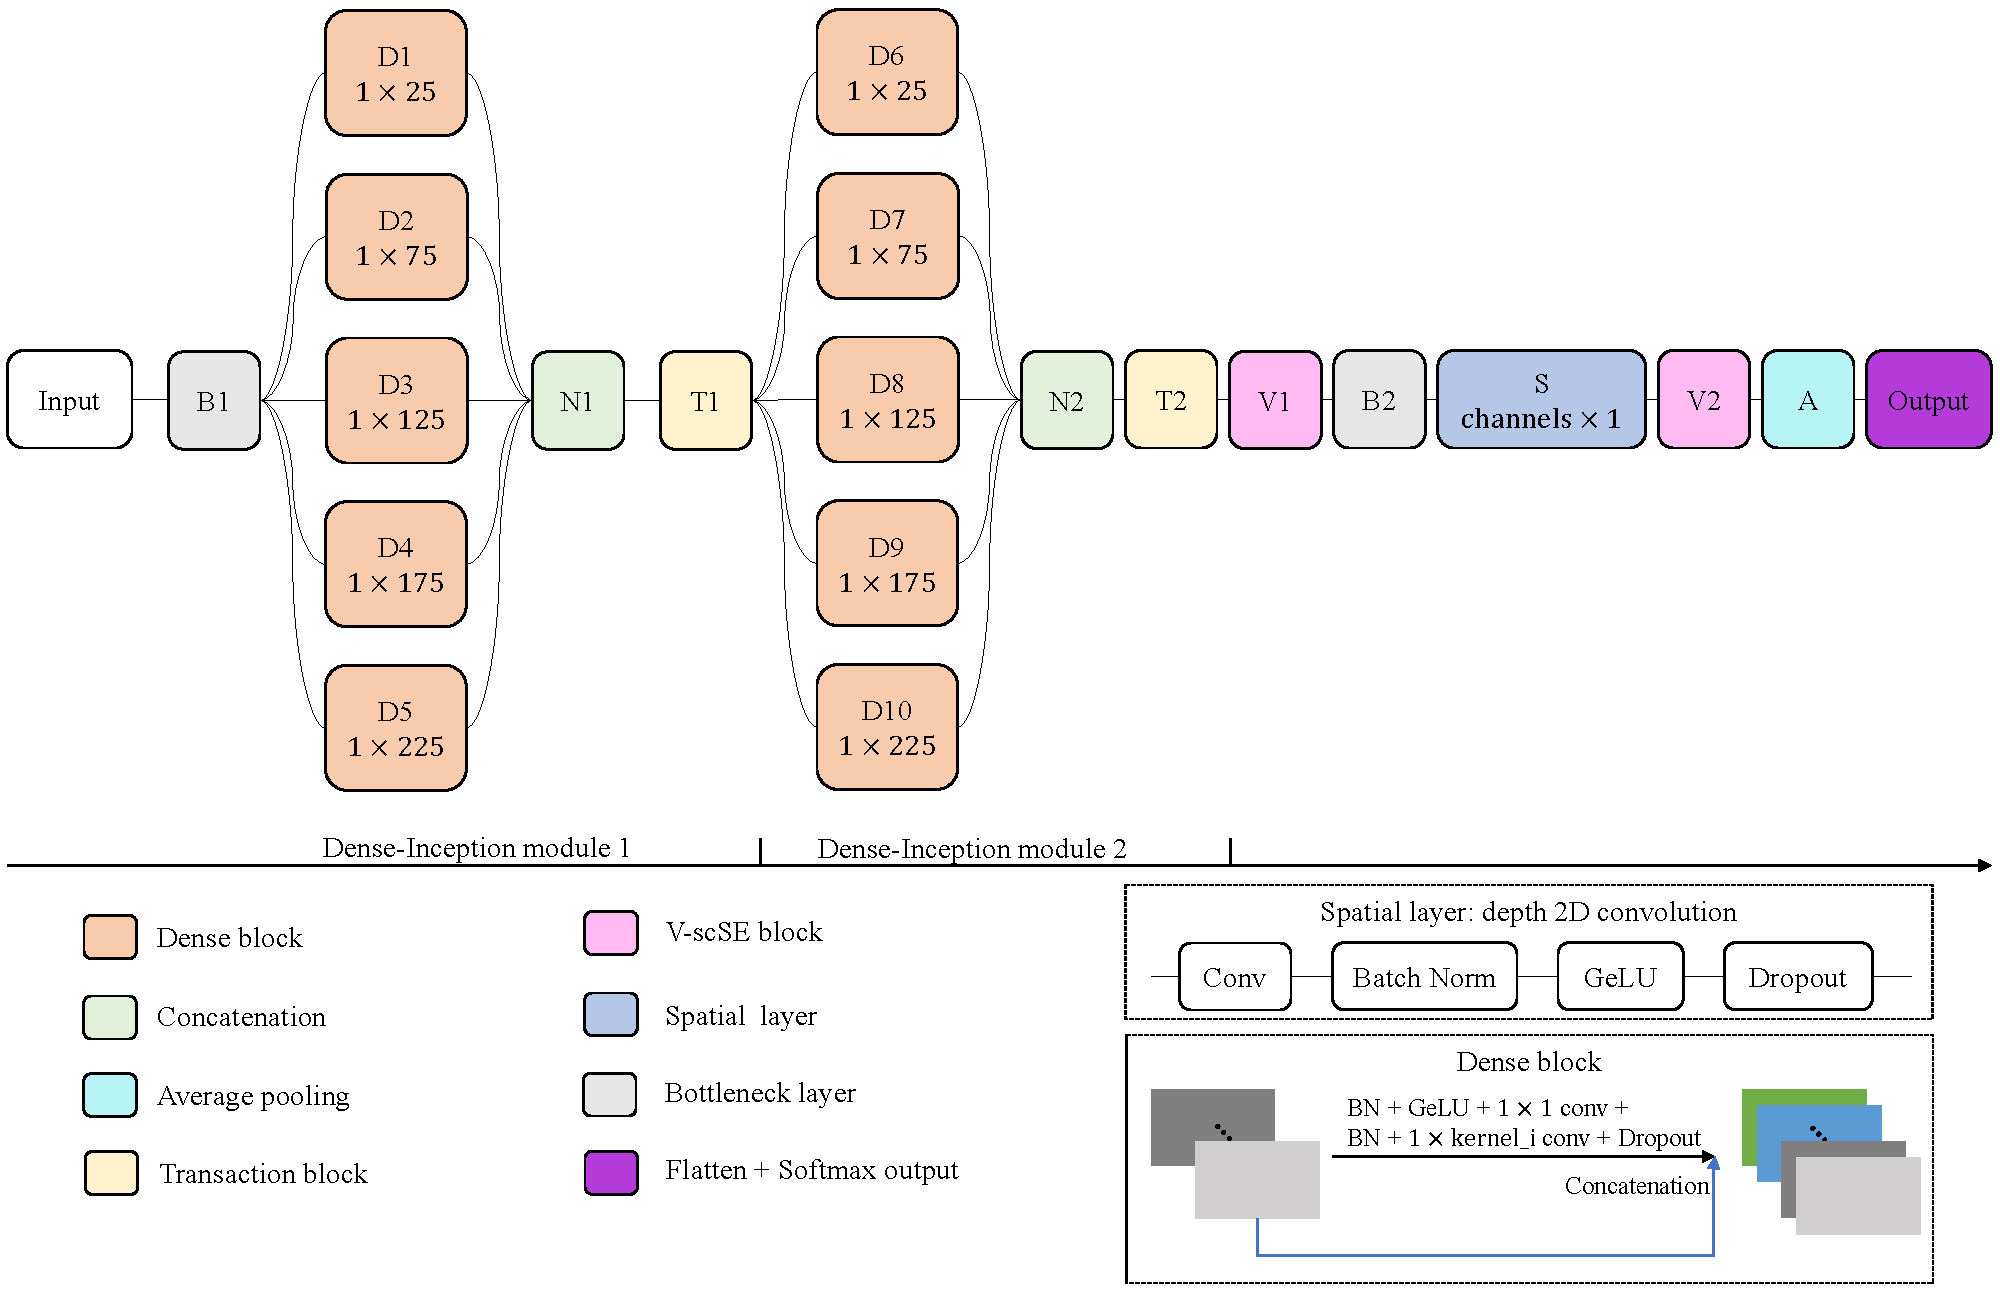
\includegraphics[width=\textwidth]{incep-dense.pdf}
  \caption{DI-VSNet结构}
  \label{fig:incep-dense}
\end{figure}

\subsection{基于Transformer构建并行分支}

卷积神经网络中,尽管卷积层因其局部感受野能够出色地捕获信号中的局部时空特征,但对于那些跨越较长时间跨度和空间分布的复杂交互信息,其建模能力受限。而Transformer模型\cite{vaswani2017attention}因其自注意力机制(Self-Attention)可以在不考虑输入位置顺序的情况下,灵活地捕捉并编码任意两点之间的相互依赖关系,从而能够更有效地理解和处理长距离依赖,但与此同时,其可能无法充分提取局部时空特征。因此,论文选择将两者进行结合,用于MI-EEG分类任务。

原始的Transformer模型是编码器-解码器(Encoder-Decoder)结构,编码器模块负责接收输入序列,并通过自注意力机制捕捉并整合整个序列中的语义和上下文信息;解码器则依据这些编码后的信息逐步生成对应的输出序列。在MI-EEG分类任务中,不涉及目标序列的生成,因此只需要使用Transformer的编码器,其结构如图~\ref{fig:encoder}~所示。
\begin{figure}
    \centering
    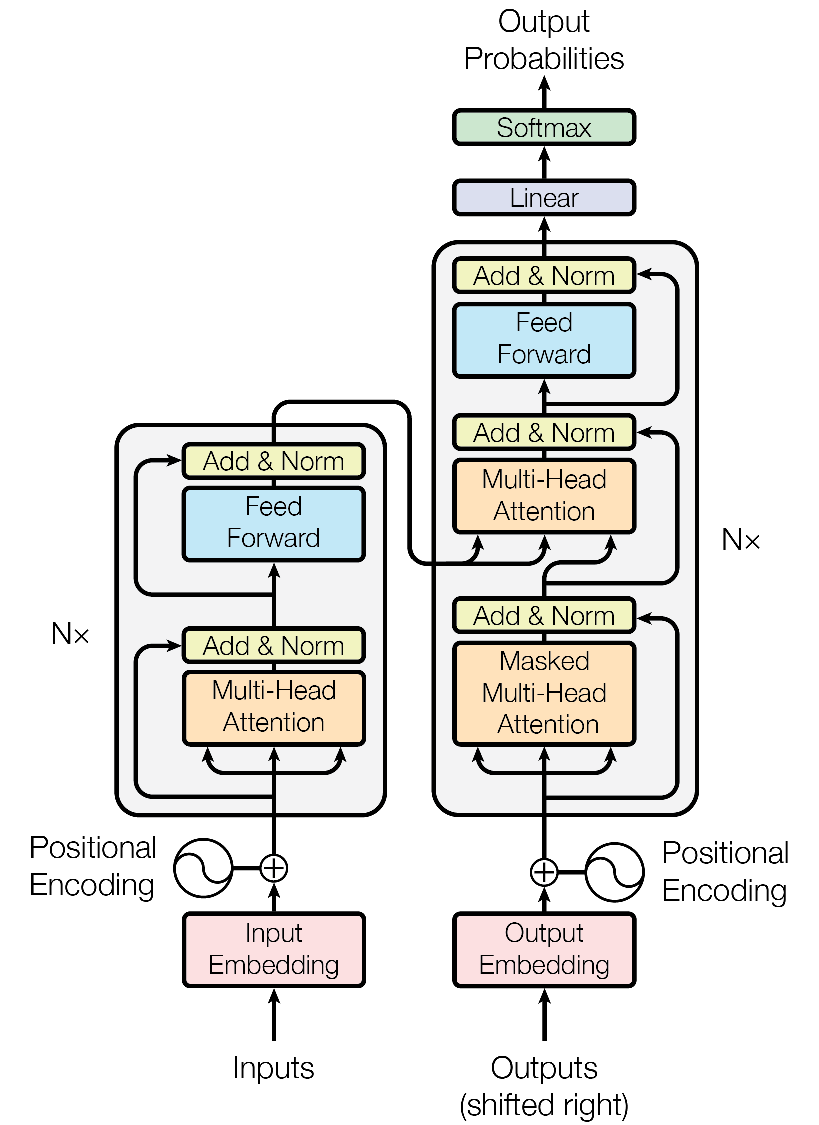
\includegraphics[height=0.7\textwidth]{encoder.pdf}
    \caption{Transformer Encoder结构}
    \label{fig:encoder}
\end{figure}
编码器由以下几部分组成:

(1) 输入嵌入与位置编码层(Input Embedding \& Positional Encoding):将输入序列转化为稠密向量表示,通过位置编码为输入添加位置信息。

(2) 多头注意力(Multi-Head Attention):使用多个并行运行的自注意力(Self-Attention)子层(头),提取不同尺度的长距离依赖,对输入进行注意力加权。

(3) 残差连接与层归一化(Add \& Norm):在每个子层之后应用残差连接与层归一化,提高模型训练效率和稳定性,避免网络退化。

(4) 前馈神经网络(Feed Forward):全连接神经网络,对多头注意力的输出进行非线性转换。

对于MI-EEG信号而言,空间维度的特征反映了电极位置特异性,时间维度的特征则体现了与事件相关去同步(ERD)和事件相关同步(ERS)等生理现象相关的时序变化。因此,重要的长依赖关系主要存在于在时间维度,即时序特征。因此,论文使用的Transformer模块沿袭经典Transformer结构。

为了更好地获取时序长依赖,将一个输入样本 \(X \in \mathbb{R}^{C \times T}\) 中的第 \(i\) 个时间序列视为一个Token \(x_i \in \mathbb{R}^{T}\),则一个样本需要 \(C\) 个Transformer处理,表达为:
\begin{equation}\label{eq:multi-trans}
    f(X)={\textstyle \sum_{i}^{C}}f_i(x_i)
\end{equation}。
其中,\(C\) 代表数据的通道数, \(T\) 代表时间序列长度。考虑单个Transformer,获得其对应的 \(x\) 的词嵌入表示 \(E \in \mathbb{R}^{T \times d_model}\) ,其中,\(d_model\) 为词嵌入维度,随后对Token \(E\) 的处理过程如下:

首先,为了编码序列的位置信息,论文对 \(E\) 进行可学习位置编码,即通过一个可学习的参数矩阵表征Token的位置信息,将其记为\(PE\),通过相加的方式与Token相融合,获得最终的Token \,\(Y\): \(Y=E+PE\)。

随后,对于 \(Y\),通过含多个自注意力机制的多头注意力层(MHA)进行处理。对于第 \(i\) 个头(head),首先通过三组线性变换,获得Query \(Q_i\),Key \(K_i\),Value \(V_i\),如公式~\ref{eq:change}所示:
\begin{equation}\label{eq:change}
    Q=W^{Q}_iY,\,K=W^{K}_iY,\,V=W^{V}_iY
\end{equation}
其中,\(W^{Q}_i,\,W^{K}_i,\,W^{V}_i \in \mathbb{R}^{d_model \times d_k}\),\(d_k=d_model \div h\),\(h\)是head的数量。通过公式~\ref{eq:sa}~得到当前head的输出,记为\(A_i\):
\begin{equation}\label{eq:sa}
    A_i=softmax(\frac{Q_iK^{T}_i}{\sqrt{d_k}}V_i)
\end{equation}
随后,根据公式~\ref{eq:mha}~对所有head的结果进行合并:
\begin{equation}\label{eq:mha}
    MHA(Y)=Concat(A_1,...,A_h)W^{O}
\end{equation}
其中,\(W^{O} \in \mathbb{R}^{T \times d_model}\),输出经过残差连接和层归一化:
\begin{equation}\label{eq:rl}
    Z=LayerNorm(Y+MHA(Y))
\end{equation}

MHA的输出会在全连接前馈神经网络(FFN)中进行转换,并同样经过残差连接和层归一化,由公式~\ref{eq:ffn}得到最终的输出。
\begin{equation}\label{eq:ffn}
    \hat{Z}=LayerNorm(Z+FFN(Z))
\end{equation}

论文从深度残差收缩网络(Deep Residual Shrinkage Network,DRSN)\cite{zhao2019deep}中得到启发,对于具有低信噪比的EEG数据,将软阈值函数(Soft Thresholding)引入Transformer中。软阈值函数是信号处理中常用的去噪方式\cite{wright2009sparse},其公式如下:
\begin{equation}\label{eq:soft}
    y=\left\{
    \begin{aligned}
    & x-\tau, \; x>\tau \\
    & \quad0, \quad -\tau \le x \le \tau \\ 
    & x+\tau, \; x<-\tau
\end{aligned}
\right.
\end{equation}
其中,\(x\) 为输入,\(y\) 为输出,\(\tau\) 为阈值。
软阈值函数将绝对值小于阈值的输入转为零值,同时对绝对值接近阈值的输入有抑制作用,从而能够减少噪声对特征的影响。论文在Transformer模块之后添加软阈值函数,通过公式~\ref{eq:tau}~计算阈值 \(\tau\):
\begin{equation}\label{eq:tau}
    \tau=\alpha \times Average(\hat{Z}),\quad \alpha \in (0,\,1)
\end{equation}
其中,\(\alpha\) 是一个可供学习的参数。通过这种方式,
\(\tau\) 是一个不太大的正数,从而避免输出全部为零的情况。

不同于Song等人将Transformer嵌入卷积神经网络之后的方式\cite{song2022eeg},论文选择以并行分支的形式引入Transformer模块。这是因为直接在卷积层之后加入Transformer可能导致模型仅能捕捉到深层卷积特征图的依赖关系,而非充分利用全局信息。并行分支的设计旨在全面利用Transformer对全局依赖的建模能力,同时避免干扰卷积神经网络本身的局部特征提取功能。

将Transformer模块引入DIS-Net后获得的新模型命名为HIT-Net,其结构如图~\ref{fig:HIT}~所示。为了综合CNN和Transformer提取的特征信息,将二者获取的特征图在深度维度进行特征聚合,因此,有必要对数据进行一定的处理,使得两个分支的数据形状相匹配。论文设计了CT-Block和TC-Block用于并行分支数据的交互融合。在CT-Block中,数据通过时间维度的池化和通道维度的卷积进行下采样,将一个样本 \(X \in \mathbb{R}^{C \times T}\) 沿通道维度压缩至 \(X^{'} \in \mathbb{R}^{C^{'} \times T}\) ,其中, \(C\) 代表通道数(电极数), \(T\) 代表时间序列长度,\(C^{'}\) 是一个大于等于1且小于等于 \(C\) 的整数,通常设定为 \(\left\lfloor \frac{C}{N} \right\rfloor\),\(N\) 为输出类别数量,这样设计的目的是减少计算开销和保留一定的空间特征信息。在TC-Block中,则通过反卷积对Transformer模块的输出进行重建,将时间维度和通道维度上采样至与CNN分支相同的大小。

\section{基于HIT-Net轻量化的端到端MI-EEG分类网络HIT-lightNet}

考虑到BCI系统对即时响应具有较高的要求,虽然HIT-Net已运用了瓶颈层、深度可分离卷积等手段有效地缩减了模型参数量,但为了追求更加卓越的实时性能表现,仍有进行进一步轻量化的必要。HIT-Net模型参数的主要来源在于Transformer模块和密集连接模块。针对Transformer模块的轻量化策略包括但不限于减少原始层级数目、量化参数类型及运用知识蒸馏技术。然而,面对小样本规模的EEG信号数据集,由于缺乏足够的大数据训练支撑,论文主要采取了减少原始层数这一轻量化途径。具体来说,对于CT-Block设计了更为高效的下采样方案,将原本由多个Transformer单元组成的Transformer分支精简为仅包含一个Transformer单元。与此同时,对于密集连接模块以及其他卷积层,论文进行针对性的轻量化卷积设计,并将在下文中对轻量化卷积模块的设计思路与方案加以阐述。

\subsection{经典轻量级网络结构}

MobileNet\cite{howard2017mobilenets}由Google团队提出,其核心思想在于引入了深度可分离卷积(Depthwise Separable Convolution),通过深度卷积处理单个输入通道,然后使用点积卷积(也称为逐点卷积或1x1卷积)跨通道整合信息。这种分解大幅减少了计算成本和模型大小,同时保持了较高的精度。在V2版本中,引入了反转残差(Inverted Residual)结构\cite{sandler2018mobilenetv2},不同于常规残差块的设计,它在网络较窄的地方采用线性瓶颈层增加深度,而非在宽度较大的地方。此外,MobileNetV2取消了线性瓶颈层后的小维度特征上的ReLU激活函数,以此来保持更多的非线性表达能力。V3版本在前两代的基础上,通过结合人类专家指导的网络设计原则与自动化的网络结构搜索(Network Architecture Search,NAS)技术\cite{howard2019searching},进一步定制了模型结构,即每个卷积层的具体通道数和操作类型都根据NAS的结果确定。此外,MobileNetV3还引入了Hard Swish这一新的激活函数以及其他的优化策略。

ShuffleNet\cite{zhang2018shufflenet}由旷视科技的研究团队所开发,其设计目标在于实现模型计算效率与预测准确性的均衡优化。为了解决分组卷积可能导致的组间特征孤立问题,ShuffleNet引入了通道混洗(Channel Shuffle)技术,即在执行完分组卷积之后,对各组内的特征图进行有序重组,以促进不同组间的特征信息相互交织和传播,从而增强模型的特征表达能力。此外,ShuffleNet针对分组卷积的配置进行了精细化调整,科学地配置组的数量和各组内的通道数,以便在有限的计算资源条件下最大限度地提升模型性能。在V2\cite{ma2018shufflenet}版本中,研究团队提出了一套高效卷积神经网络设计原则,并据此对ShuffleNetV1架构做出了改进。他们摒弃了1 \times 1的分组卷积操作,转而采用通用卷积来替代,并提出了通道分割(Channel Split)策略。具体而言,模型将输入特征图均匀划分为两个部分,一部分不经额外计算直接向下传输,另一部分则经历一系列计算后再与前者合并。在concatenate操作之后,继续实施通道混洗操作,从而有效提升模型在轻量化条件下的性能表现。ShuffleNet的结构如图~\ref{fig:shufflenet}~所示,图~\ref{fig:shufflenet}~(a)是ShuffleNet的基本单元,图~\ref{fig:shufflenet}~(b)在ShuffleNet基本单元的基础上增加了下采样,图~\ref{fig:shufflenet}~(c)是ShuffleNetV2的基本单元,图~\ref{fig:shufflenet}~(d)在ShuffleNetV2基本单元的基础上增加了下采样。
\begin{figure}
    \centering
    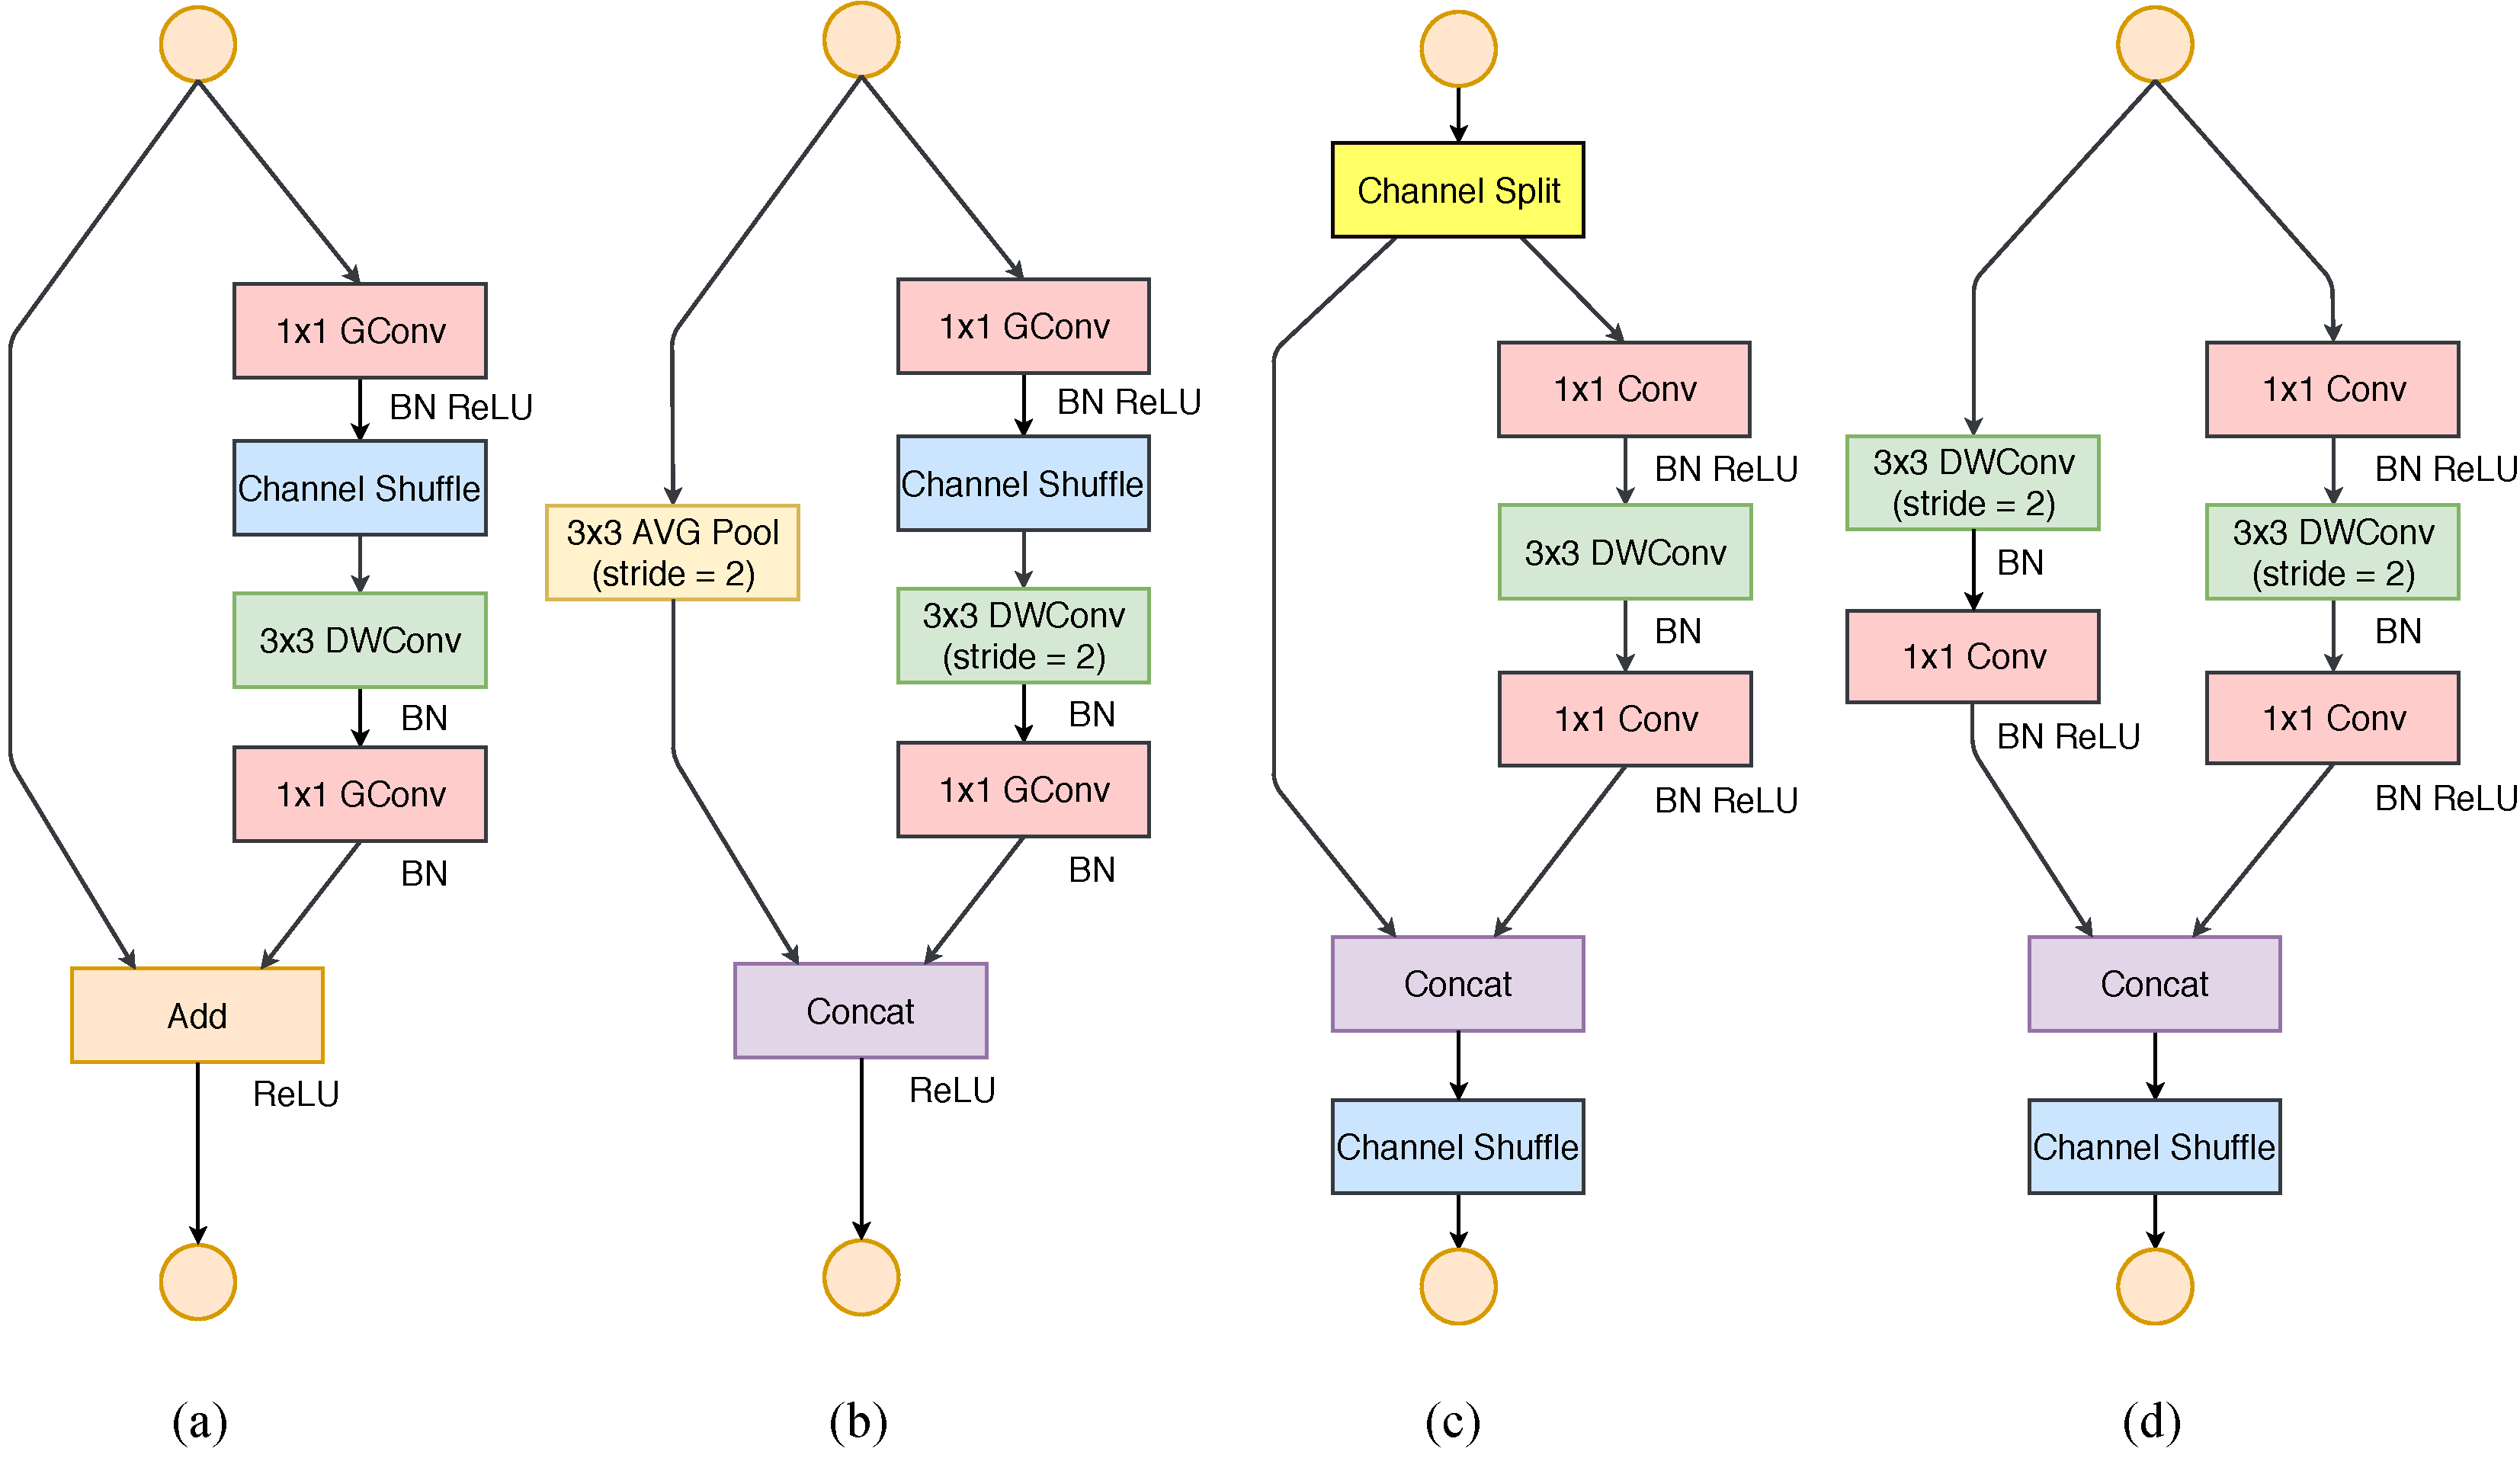
\includegraphics[width=\textwidth]{shufflenet.pdf}
    \caption{ShuffleNet结构}
    \label{fig:shufflenet}
\end{figure}

GhostNet\cite{han2020ghostnet}由华为诺亚方舟实验室提出,其核心思想在于提出了幻影模块(Ghost Module),该模块针对深度神经网络中存在的潜在冗余和相关性较高的特征图问题,通过高效的计算策略提炼出“幻影特征图”。研究团队发现,在许多情况下,多个特征图可能蕴含着相似的模式信息,这意味着部分特征图的信息实质上可以从其他特征图中推衍得出,犹如“幻影”。鉴于此,GhostNet摒弃了对每组特征图均采用标准卷积的传统做法,转而采用一种更为经济高效的计算方式去合成这类“幻影特征图”。在具体实施中,首先运用有限数量的标准卷积层提取基础特征图,以此严格控制参数规模,接下来通过对基础特征图施加一组精心设计的线性变换(通常是深度可分离卷积中的逐点卷积操作),高效地生成大量辅助特征图,这些辅助特征图被视为原始特征图的“幻影”。最后,Ghost模块将“幻影特征图”与标准卷积产生的少量核心特征图整合在一起,以有效模拟传统卷积所带来的丰富表征能力,在保持高精度的同时,降低了模型的计算复杂性和参数规模。Ghost模块的结构如图~\ref{fig:ghost}~所示,其中,Identity操作由标准卷积生成的特征图,\(\Phi\) 为廉价线性变换。
\begin{figure}
    \centering
    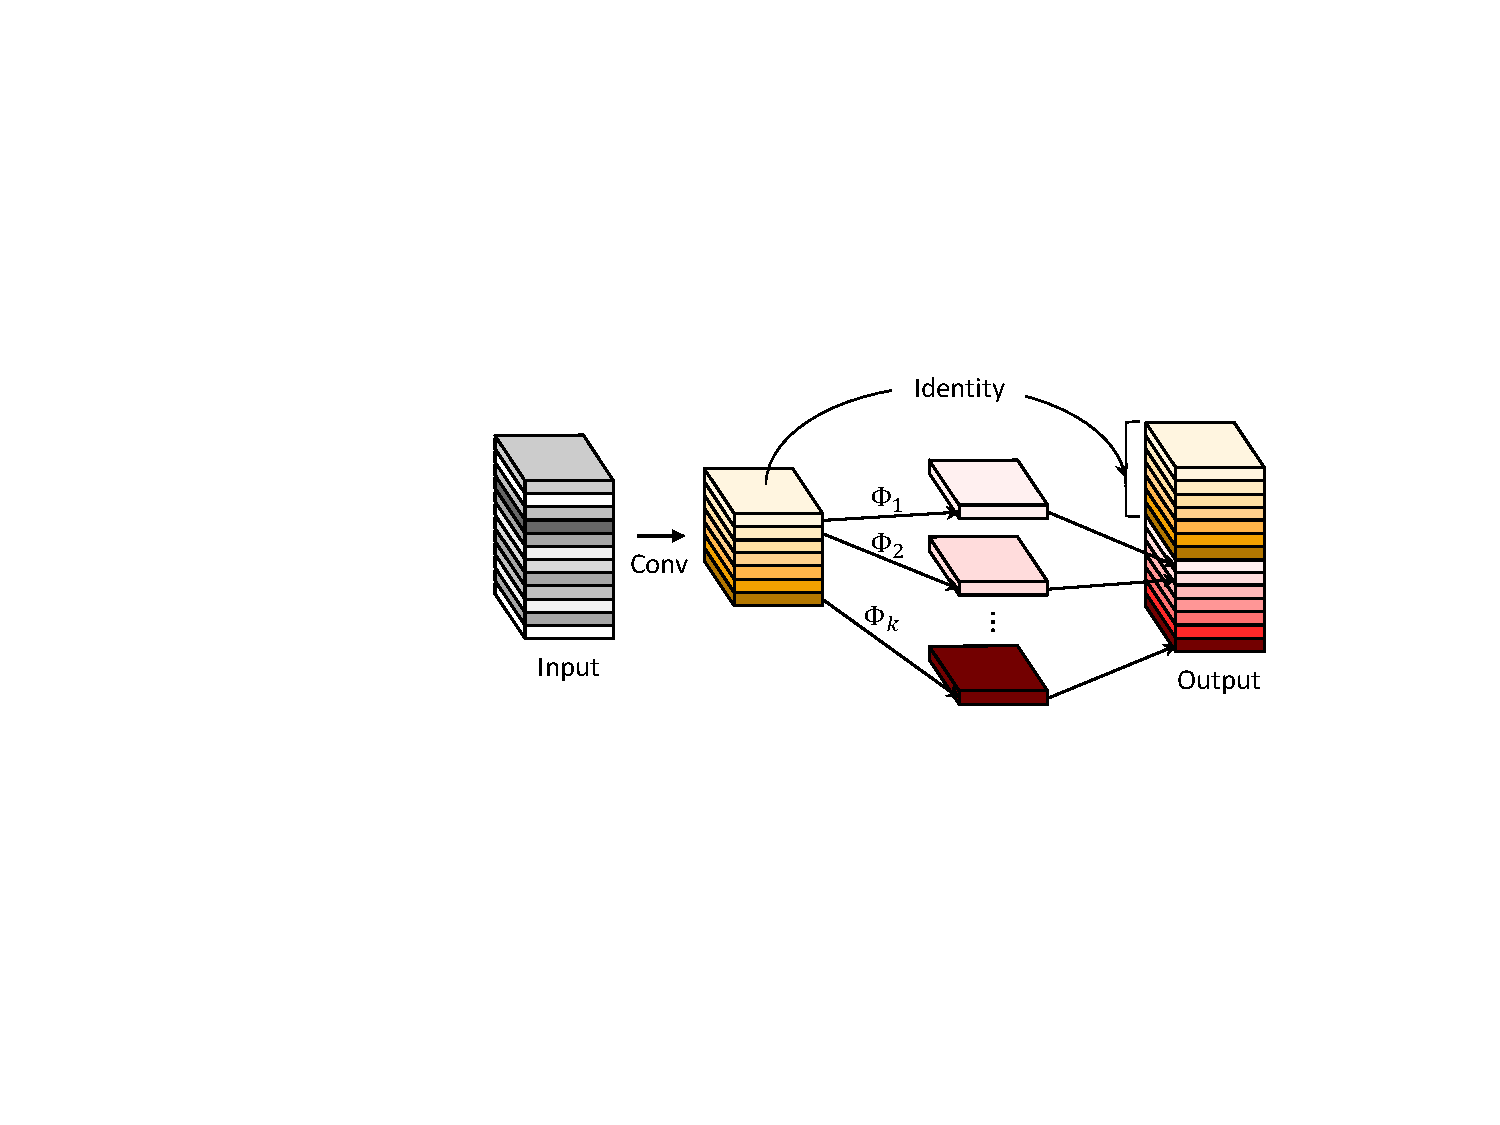
\includegraphics[width=\textwidth]{ghost.pdf}
    \caption{Ghost模块结构}
    \label{fig:ghost}
\end{figure}

\subsection{ShuffleNet结合GhostNet的轻量化卷积模块}

在HIT-Net架构中,已应用了诸如瓶颈层设计以及深度可分离卷积技术,从而有效地压缩了模型参数量。因此,本节在现有成果的基础上,主要结合ShuffleNetV2的基础单元和GhostNet所提出的Ghost模块进行了针对性改良。

ShuffleNetV2的优势体现在其利用通道混洗操作促进不同特征图组之间的信息交互,特别是在Channel Split机制中,它将特征图分割成两个部分,其中一个部分不经额外计算直接向下进行传递,这种设计有助于减少模型分支内的参数量。然而,ShuffleNetV2在进行Channel Split时,通常是对特征图进行均匀划分,这种方式难以灵活调整直传特征图的比例,可能导致对重要特征信息的有效利用率不足,并且在极端情况下可能影响模型精度。此外,ShuffleNetV2的基础结构在深度维度上的特征变换主要依赖于1×1卷积,这在一定程度上限制了其内在的深度特征变换能力。

为了提升ShuffleNetV2基本模块在深度特征变换方面的能力,论文提出了一种可调节分支比例的Shuffle模块(Adaptive Shuffle Module, AS模块),其架构如图(a)所示。假设卷积层的输入深度为 \(D_{in}\),输出深度为 \(D_{out}\),针对不同的输入输出深度关系(即 \(D_{in} \le D_{out}\) 和 \(D_{in} > D_{out}\) ),论文对AS模块进行了优化,分别形成了图(b)所示的GAS模块(Growing Adjustable Shuffle Module)和图(c)所示的SAS模块(Straight Adjustable Shuffle Module)。

对于GAS模块,在保留原有直接传递分支的同时,对进行深度变换的分支进行了如下改进:根据采样频率特性调整卷积核大小,为了描述的简洁性,以时间域特征提取卷积模块为例,并将其卷积核大小设定为1 \times 25,对于采样频率为250Hz的BCI Competition IV Dataset 2A数据集而言,意味着该卷积核以0.1秒的时间窗口进行特征捕获。进入变换分支的特征图首先通过1 \times 1卷积实现深度变换,紧接着通过1 \times 25的深度卷积进行特征提取,最后再次通过1 \times 1卷积将深度变换至输出需要的深度。在此过程中,加入了批归一化和GeLU激活函数。这样设计的目的是优化GAS模块对MI-EEG分类任务的性能。

对于权重参数为 \(ratio\) 的GAS模块,其直接传递分支的特征图输入数量 \(BS_{in}\) 设定为 \(BS_{in} = D_{in} \times ratio\),对应的输出数量 \(BS_{out}\) 同样为 \(BS_{out} = D_{in} \times ratio\)。而变换分支的特征图输入数量\(BT_{in}\) 则设定为 \(BT_{in} = D_{in} - BS_{in}\),其输出特征图数量 \(BT_{out}\) 计算为 \(BT_{out} = D_{out} - BS_{out}\)。这样的设计使得GAS模块能在维持模型轻量化的同时,更精准地针对MI-EEG分类任务进行深度特征提取与整合。

为此,论文对ShuffleNetV2的基础模块进行改进,提出了一种AS模块(Adjustable Shuffle Module),其结构如图(a)所示。令卷积层输入深度为 \(D_{in}\),输出深度为 \(D_{out}\),为了增强AS模块的深度特征变换能力,论文针对 \(D_{in} \le D_{out}\) 和 \(D_{in} > D_{out}\) 的情况对Shuffle模块进行了进一步改进,其结构分别如图(b)和图(c)所示,命名为GAS模块和SAS模块。其直接传递分支的特征图输入数量 \(BS_{in}\) 设定为 \(BS_{in} = D_{in} \times ratio\),对应的输出数量 \(BS_{out}\) 同样为 \(BS_{out} = D_{in} \times ratio\)。而变换分支的特征图输入数量\(BT_{in}\) 则设定为 \(BT_{in} = D_{in} - BS_{in}\),其输出特征图数量 \(BT_{out}\) 计算为 \(BT_{out} = D_{out} - BS_{out}\)。这样的设计使得GAS模块能在维持模型轻量化的同时,更精准地针对MI-EEG分类任务进行深度特征提取与整合。

在GAS模块中,对直接向下传递的分支不做修改,而对进行变换的分支做以下修改:修改卷积核大小为与采样频率相关,为了简洁起见,设置为时间提取卷积模块,卷积核大小设定为1\times25,对于BCI Competition IV Dataset 2A数据集而言,采样频率为250Hz,25大小的卷积核代表基于0.1s的采样周期进行特征提取。进入变换分支的特征图首先通过1\times1卷积进行升维,随后经过1\times25的深度卷积进行特征提取,在这个过程中,加入了批归一化与GeLU激活函数。这样做的目标是针对MI-EEG分类任务进行优化。对于权重参数为 \(ratio\) 的GAS模块,其直接传递分支的特征图输入数量 \(BS_{in}\) 为 \(BS_{in} = D_{in} \times ratio\),输出数量 \(BS_{out}\) 为 \(BS_{out} = D_{in} \times ratio\),变换分支的特征图输入数量 \(BT_{in}\) 为 \(BT_{in} = D_{in} - BS_{in}\),输出特征图数量为 \(BT_{out}\) 为 \(BT_{out} = D_{out} - BS_{out}\)。

\section{基于MEKT算法改进的MI-EEG迁移学习算法SV-MEKT}

